%  compress using: gs -sDEVICE=pdfwrite -dCompatibilityLevel=1.4 -dNOPAUSE -dQUIET -dBATCH      -sOutputFile=foo-ShapingSwarmCompressed.pdf ShapingSwarmFrictionSharedInput.pdf

%\documentclass[conference]{IEEEtran}
\documentclass[letterpaper, 10 pt, conference]{ieeeconf}
\IEEEoverridecommandlockouts% This command is only needed if 
                                                          % you want to use the \thanks command
%\overrideIEEEmargins                                      % Needed to meet printer requirements.
\usepackage{times}


\makeatletter 
\let\NAT@parse\undefined
\makeatother

% numbers option provides compact numerical references in the text. 
%\usepackage[numbers]{natbib}
\usepackage{multicol}
\usepackage[bookmarks=true]{hyperref}

\usepackage{bbm}
\usepackage{calc}
\usepackage{url}
\usepackage{transparent}
\usepackage{hyperref}
\hypersetup{
  colorlinks =false,
  urlcolor = black,
  linkcolor = black
}
\usepackage{graphicx}
\usepackage[cmex10]{amsmath}
\usepackage{bm}
\usepackage{amssymb}
\usepackage{rotating}

\usepackage{chngcntr}
\counterwithin{paragraph}{subsection} % makes paragraph depend on subsection


%\usepackage{xfrac}
\usepackage{nicefrac}
\usepackage{cite}
\usepackage[caption=false,font=footnotesize]{subfig}
\usepackage[usenames, dvipsnames]{color}
\usepackage{colortbl}
%\usepackage{caption}

%\usepackage{wrapfig}
\usepackage{overpic}
%\usepackage{subfigure}
%\usepackage{textcomp}
\graphicspath{{./pictures/pdf/},{./pictures/ps/},{./pictures/png/},{./pictures/jpg/}}
\usepackage{breqn} %for breaking equations automatically
\usepackage[ruled]{algorithm}
\usepackage{algpseudocode}
%\usepackage{algorithmic}
\usepackage{multirow}
\usepackage{todonotes}
\usepackage{authblk}
\usepackage[per-mode=symbol, detect-weight=true, binary-units=true]{siunitx}
\usepackage{rotating}
%\newcommand{\todo}[1]{\vspace{5 mm}\par \noindent \framebox{\begin{minipage}[c]{0.98 \columnwidth} \ttfamily\flushleft \textcolor{red}{#1}\end{minipage}}\vspace{5 mm}\par}
% uncomment this to hide all red todos
%\renewcommand{\todo}{}

%% ABBREVIATIONS
\newcommand{\qstart}{q_{\text{start}}}



%% MACROS


\providecommand{\abs}[1]{\left\lvert#1\right\rvert}
\providecommand{\norm}[1]{\left\lVert#1\right\rVert}
\providecommand{\normn}[2]{\left\lVert#1\right\rVert_#2}
\providecommand{\dualnorm}[1]{\norm{#1}_\ast}
\providecommand{\dualnormn}[2]{\norm{#1}_{#2\ast}}
\providecommand{\set}[1]{\lbrace\,#1\,\rbrace}
\providecommand{\cset}[2]{\lbrace\,{#1}\nobreak\mid\nobreak{#2}\,\rbrace}
\providecommand{\lscal}{<}
\providecommand{\gscal}{>}
\providecommand{\lvect}{\prec}
\providecommand{\gvect}{\succ}
\providecommand{\leqscal}{\leq}
\providecommand{\geqscal}{\geq}
\providecommand{\leqvect}{\preceq}
\providecommand{\geqvect}{\succeq}
\providecommand{\onevect}{\mathbf{1}}
\providecommand{\zerovect}{\mathbf{0}}
\providecommand{\field}[1]{\mathbb{#1}}
\providecommand{\C}{\field{C}}
\providecommand{\R}{\field{R}}
\newcommand{\Cspace}{\mathcal{Q}}
\newcommand{\Uspace}{\mathcal{U}}
\providecommand{\Fspace}{\Cspace_\text{free}}
\providecommand{\Hcal}{$\mathcal{H}$}
\providecommand{\Vcal}{$\mathcal{V}$}
\DeclareMathOperator{\conv}{conv}
\DeclareMathOperator{\cone}{cone}
\DeclareMathOperator{\homog}{homog}
\DeclareMathOperator{\domain}{dom}
\DeclareMathOperator{\range}{range}
\DeclareMathOperator{\sign}{sgn}
\providecommand{\polar}{\triangle}
\providecommand{\ainner}{\underline{a}}
\providecommand{\aouter}{\overline{a}}
\providecommand{\binner}{\underline{b}}
\providecommand{\bouter}{\overline{b}}
\newcommand{\D}{\nobreakdash-\textsc{d}}
%\newcommand{\Fspace}{\mathcal{F}}
\providecommand{\Fspace}{\Cspace_\text{free}}
\providecommand{\free}{\text{\{}\mathsf{free}\text{\}}}
\providecommand{\iff}{\Leftrightarrow}
\providecommand{\subinner}[1]{#1_{\text{inner}}}
\providecommand{\subouter}[1]{#1_{\text{outer}}}
\providecommand{\Ppoly}{\mathcal{X}}
\providecommand{\Pproj}{\mathcal{Y}}
\providecommand{\Pinner}{\subinner{\Pproj}}
\providecommand{\Pouter}{\subouter{\Pproj}}
\DeclareMathOperator{\argmax}{arg\,max}
\providecommand{\Aineq}{B}
\providecommand{\Aeq}{A}
\providecommand{\bineq}{u}
\providecommand{\beq}{t}
\DeclareMathOperator{\area}{area}
\newcommand{\contact}[1]{\Cspace_{#1}}
\newcommand{\feasible}[1]{\Fspace_{#1}}
\newcommand{\dd}{\; \mathrm{d}}
\newcommand{\figwid}{0.22\columnwidth}
\newcommand{\TRUE}{\textbf{true}}
\newcommand{\FALSE}{\textbf{false}}
\newcommand{\xupdownarrow}[1]{%
  {\left\updownarrow\vbox to #1{}\right.\kern-\nulldelimiterspace}
}
%\newcommand{\xleftrightarrow}[1]{%
%  {\left\leftrightarrow\vbox to #1{}\right.\kern-\nulldelimiterspace}
%}
\DeclareMathOperator{\atan2}{atan2}
\allowdisplaybreaks

\newtheorem{theorem}{Theorem}
\newtheorem{definition}[theorem]{Definition}
\newtheorem{lemma}[theorem]{Lemma}


\pdfinfo{
   /Author (Shiva Shahrokhi and Aaron T. Becker)
   /Title  (Algorithms for Shaping a Particle Swarm with a Shared Input by Exploiting Non-Slip Wall Contacts)
   /CreationDate (D:20160129120000)
   /Subject (Simple Robots)
   /Keywords (Robots;Uniform Control Inputs)
}


% paper title
\title{\LARGE \bf Exploiting Non-Slip Wall Contacts \\  to Position Two Particles Using The Same Control Input}

% You will get a Paper-ID when submitting a pdf file to the conference system
\author{Shiva Shahrokhi, Jingang Shi,  Benedict Isichei, and Aaron T. Becker% <-this % stops a space
\thanks{*This work was supported by the National Science Foundation under Grant No.\ \href{http://nsf.gov/awardsearch/showAward?AWD_ID=1553063}{ [IIS-1553063]} and \href{http://nsf.gov/awardsearch/showAward?AWD_ID=1619278}{[IIS-1619278]}.}% <-this % stops a space
\thanks{Authors are with the Department of Electrical and Computer Engineering,  University of Houston, Houston, TX 77204 USA        {\tt\small  \{sshahrokhi2,atbecker\}@uh.edu}}%
}
%\affil{Department of Electrical and Computer Engineering, \\
% University of Houston, Houston, TX 77204-4005 USA\\
% {\tt\small  \{sshahrokhi2, aviswanathanmahadev, atbecker\}@uh.edu}}
%\thanks{S. Shahrokhi, A. Mahadev and  A. Becker are with the Department of Electrical and Computer Engineering,  University of Houston, Houston, TX 77204-4005 USA {\tt\small  \{sshahrokhi2, aviswanathanmahadev, atbecker\}@uh.edu}
%}
%} %\end thanks

\begin{document}



\maketitle
\thispagestyle{empty}
\pagestyle{empty}


\begin{abstract}


Steered particles offer a method for targeted therapy, interventions, and drug delivery in regions inaccessible by large robots.
Magnetic actuation has the benefits of requiring no tethers, being able to operate from a distance, and in some cases allows imaging for feedback (e.g. MRI).
 This paper investigates control with uniform magnetic gradients (the same force is applied everywhere in the workspace).
Given three orthogonal magnetic fields, steering one particle in 3D is trivial. 
Adding additional particles to steer makes the system underactuated because there are more states than control inputs. 
However, the walls of in vivo and artificial environments often have surface roughness such that the particles do not move unless actuation pulls them away from the wall.
In previous works, we showed that the individual 2D position of two particles is controllable in a square workspace with non-slip wall contact. 
Because in vivo environments are usually not square, this work extends the previous work to convex workspaces including circles and 3D positioning. 
This paper also implements the algorithms using a hardware setup inspired by gastrointestinal tract.




%There are driving applications for large populations of tiny robots in robotics, biology, and chemistry.
%These robots often lack onboard computation, actuation, and communication.
%Instead, these ``robots''  are  particles carrying some payload and the particle swarm is controlled by a shared control input such as a uniform magnetic gradient or electric field.
%In previous works, we showed that the 2D position of each particle in such a swarm is controllable if the workspace contains a single obstacle the size of one particle.
%In previous works, we showed that the individual 2D position of two particles in such a swarm is controllable in a rectangular workspace requiring non-slip wall contact. However, both in vivo and artificial environments are usually not rectangular. 
%This work extends that work to any polygonal workspace, and focus on extending the algorithm for circular workspaces. Then it extends the algorithm to 3D. Results are validated with simulations and with a magnetic setup using two steel half a millimeter balls.
%This work extends the analysis to convex workspaces and 3D positioning. This paper also implements the algorithms using a hardware setup inspired by intestine anatomy.
%Requiring a small, rigid obstacle suspended in the middle of the workspace is a strong constraint, especially in 3D.
%Often particles are placed into an em
%This paper relaxes that constraint, and provides position control algorithms that only require non-slip wall contact in 2D.
%Both in vivo and artificial environments often have such boundaries.
%We assume that particles in contact with the boundaries have zero velocity if the shared control input pushes the particle into the wall.
%This paper provides a shortest-path algorithm for positioning a two-particle swarm, and a generalization to positioning an $n$-particle swarm.
%Results are validated with simulations and a hardware demonstration.







%Consider a swarm of particles controlled by global inputs. 
%This paper presents algorithms for shaping such swarms in 2D using boundary walls.
%The range of configurations created by conforming a swarm to a boundary wall is limited. 
%We describe the set of stable configurations of a particle swarm in two canonical workspaces, a circle and a square. 
%To increase the diversity of configurations, we add boundary interaction to our model.  
%We provide algorithms using friction with walls to place two robots at arbitrary locations in a rectangular workspace.
%Next, we extend this algorithm to place $n$ agents at desired locations. 
%We conclude with efficient techniques to generate correlations of a particle swarm not possible without wall-friction. 
%Simulations %and hardware implementations with 100 robots 
%validate these results.

%These methods may have particular relevance for micro- and nano-robots controlled by global inputs.
%, whose small size limits onboard computation and power. For this reason they are usually powered and controlled by global inputs, such as a uniform external electric or magnetic field, and every robot receives the same control inputs.
%Due to their small size, large numbers of micro-robots are required to deliver sufficient payloads.
% Nevertheless, these applications require precision control of the shape and position of the robot swarm. Precision control requires breaking the symmetry caused by the global input.  

 



% KEYWORDS:   uniform control, under-actuation, particle swarm
\end{abstract}

\IEEEpeerreviewmaketitle

%%%%%%%%%%%%%%%
\section{Introduction}\label{sec:Intro}

This chapter investigates maximizing torque applied by a large number of particles, hereafter called a \emph{swarm}, when the swarm has non-slip contact with a rigid, 2D body. 
 The under-actuated swarm is steered by a shared signal that consists of a vector direction for movement. 
  The robotic system is comprised of the swarm of particles, the shared control signal, and an external sensor that measures the swarm position.
   This chapter examines analytically two representative aspects of swarm torque control: first, pushing a pivoted rod, and second pushing a free body. 
   We conclude with hardware experiments with centimeter-scale robots. Maximizing torque improves the efficiency of a particle swarm.

 

\begin{figure}
\begin{center}
	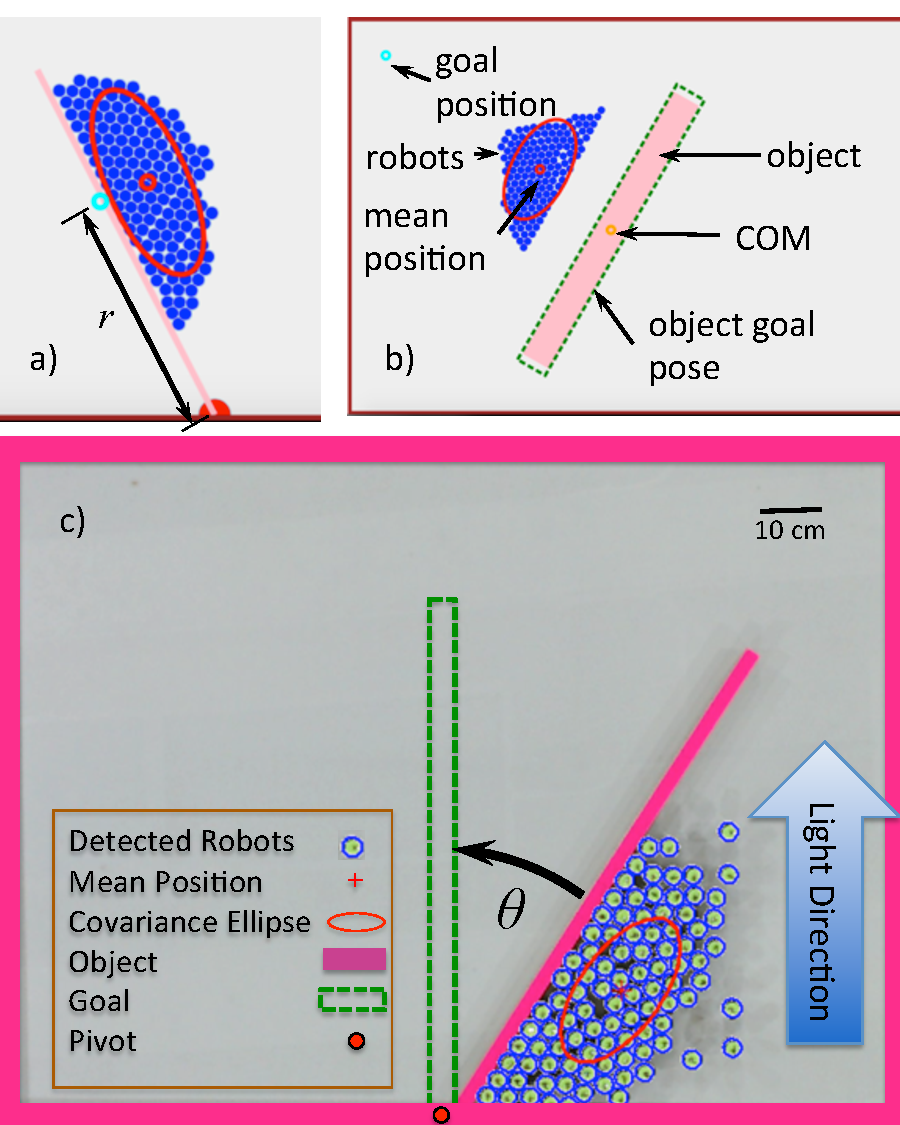
\includegraphics[width=.9\columnwidth]{CoverPhoto.pdf}
\end{center}
\vspace{-1em}
\caption{\label{fig:FirstImage}
%Torque control of an object is essential for manipulation unless objects are homogeneous discs, especially when there are narrow passageways or the objects must be aligned, e.g. sensors and emitters. 
%This paper provides the optimal position for a swarm to push to maximize torque production using a highly under-actuated system where all robots are controlled uniformly by the same input. 
(a) Simulation of robots exerting torque on a hinged ``door".
(b) Orientation control of a free long rod.
(c) Hardware robots applying torque to an object. See video attachment.% A full resolution video is available at \url{https://youtu.be/7Q5lu_ZFbxI}.
}
\vspace{-1em}
\end{figure}

With a single agent, torque control is straightforward: the agent simply maximizes the length of the movement arm to maximize torque. To make an agent push open a door, it should push on the edge furthest from the hinge. 
The optimal solution for a swarm of particles is not straightforward because they cannot all push at one position.

This chapter focuses on maximizing torque using the swarm's position distribution. 
Representative results are shown in Fig. \ref{fig:FirstImage}:  torque control using 56 mobile robots on a pivoted and a free object.




%%%%%%%%%%%%%%%
%%%%%%%%%%%%%%%

%%%%%%%%%%%%%%%%%%%%%%%%%%%%%%%%%%%%%%%%%%%%%%%%%%%%%%%%%%%
\section{Related work}\label{sec:RelatedWork}
%%%%%%%%%%%%%%%%%%%%%%%%%%%%%%%%%%%%%%%%%%%%%%%%%%%%%%%%%%%

Controlling the \emph{shape}, or relative positions, of a swarm of robots is a key ability for a range of applications.  Correspondingly, it has been studied from a control-theoretic perspective in  both centralized and decentralized approaches. For examples of each, see the centralized virtual leaders in \cite{egerstedt2001formation}, and the  gradient-based decentralized controllers  using control-Lyapunov functions in~\cite{hsieh2008decentralized}. However, these approaches assume a level of intelligence and autonomy in individual robots that exceeds the capabilities of many systems, including current micro- and nano-robots.  Current micro- and nano-robots, such as those in~\cite{Chowdhury2015,martel2015magnetotactic,Xiaohui2015magnetiteMicroswimmers} lack onboard computation.

This chapter focuses on centralized techniques that apply the same control input to both particles. 
Precision control requires breaking the symmetry caused by the uniform input.  
Symmetry can be broken using particles that respond differently to the uniform control signal, either through agent-agent reactions \cite{bertozzi2015ring}, or engineered inhomogeneity  \cite{Donald2013,bretl2007,beckerIJRR2014}. 
 The magnetic gradients of MRI scanners are \emph{uniform}, meaning the same force is applied everywhere in the workspace\cite{nosrati2018development}.
 This work assumes a uniform control with homogenous particles, as in~\cite{AaronManipulation2013}, and breaks the control symmetry using obstacles in the workspace. 

%The techniques in this paper are inspired by artificial force-fields. 

%\emph{Fluid-flow:} 
%Fluid flow along boundaries generates a shear force that pushes different parts of a body in opposing directions. 
%Most introductory fluid dynamics textbooks provide models~\citep{Munson2013}.
%Similarly, a swarm of robots under global control pushed along a boundary will experience shear forces.  
%This is a position-dependent force, and so can be exploited to control the configuration or shape of the swarm.  
% \citep{spears2006physics}~used these forces to disperse a swarm's spatial position for coverage for physics-based swarm simulations.

%\emph{Artificial Force-fields:}
%Much research has focused on generating non-uniform artificial force-fields that can be used to rearrange passive components. 
Alternative techniques rely on non-uniform inputs, such as artificial force-fields.
Applications have included techniques to design shear forces for sensorless manipulation of a single object by~\cite{lamiraux+2001:ra}.  
\cite{vose2012sliding} demonstrated a collection of 2D force fields generated by six degree-of-freedom vibration inputs to a rigid plate.  These force fields, including shear forces, could be used as a set of primitives for motion control to steer the formation of multiple objects. %However unlike the uniform control model in this paper, their control was multi-modal and position-dependent.
%\todo{talk about obstacles, think about adding goldberg}

%This paper develops control algorithms using uniform control fields, such as the magnetic resonance navigation \cite{nosrati2018development}.%field in a clinical MRI [insert a recent reference from Sylvain Martel using MRI].
Similarly, much recent work in magnet control has focused on exploiting inhomogeneities in the magnetic field to control multiple micro particles  using gradient-based pulling~\cite{Salmanipour2018EightDOF,Denasi2018independent}.  
Unfortunately, using large-scale external magnetic fields makes it challenging to independently control more than one microrobot unless the  distance between the electromagnetic coils is at the same length scales as the robot workspace~\cite{diller2016six, Denasi2018independent, Salmanipour2018EightDOF }. In contrast, % to methods that exploit inhomogeneities in the magnetic field to control multiple micro particles, e.g. \cite{Denasi2018independent}, that exploited nonlinearities generated by four magnetic coils in close proximity to the workspace to achieve trajectory control of two microspheres, 
 this chapter requires only a controllable constant gradient in orthogonal directions to position the particles.
% Systems like this one are poorly suited for PRM and RRT*-type methods\cite{lavalle2006planning} because if during a movement a collision occurs, that movement is irreversible.
   %Flow in a pipe or body lume

If a control input causes the particles to collide with obstacles at different times, inverting the control input does not undo the action. 
 Due to this lack of time-reversibility, techniques that require a bidirectional graph, e.g. PRM \cite{kavraki1996probabilistic} and RRT* \cite{lavalle2006planning} are not suitable.
  Instead, this chapter employs a greedy search strategy. 
%%%%%%%%%%%%%%%
%%%%%%%%%%%%%%%%%%%%%%%%%%%%%%%%%%%%%%%%%%%%%%%%%%%%%%%%%%%
%\section{Torque control}
%\label{sec:theory}
%%%%%%%%%%%%%%%%%%%%%%%%%%%%%%%%%%%%%%%%%%%%%%%%%%%%%%%%%%%
%\subsection{Controlling Torque}

%We derive inspiration from recent work on pulling with a swarm \cite{pulltogether}. The contribution of this work is to map swarm distributions to torque production.
%The orientation of an object's major axis is important when a swarm is manipulating a non-symmetric object through narrow corridors. 
%Orientation is controllable by applying torque to the object. 
%To change the output torque $\tau$ in~\eqref{eq:torque}, we can choose the direction and magnitude of the force applied $F$, and the moment arm from the object's center of mass (COM) $O$ to the point of contact $P$.
%We define a coordinate frame rooted at the COM, with the $x$-axis parallel to the object's longest axis. The resulting torque is:
%
%\begin{equation}
%\tau = F \times (P - O ).\label{eq:torque}
%\end{equation}
%
%We assume that the forces produced by individual particles add linearly. 
% As \cite{pulltogether} indicates, this is often a simplification of the true dynamics. 
% The swarm version of \eqref{eq:torque} is the summation of the forces contributed by $n$ individual particles:
%\begin{align}
%\tau_{\text{total}} &= \sum\limits_{i=1}^n \rho_i F_i \times (P_i - O ) \textrm{      and}   \label{eq:swarmtorque}\\
%F_{\text{total}} &= \sum\limits_{i=1}^n \rho_i F_i.  \label{eq:swarmforce}
%\end{align}
%Here $F_i$ is the force that the $i^{\textrm{th}}$ particle applies. 
%Not all particles are in contact with the object.  
%$\rho_i$ is an indicator variable: $\rho_i=1$ if the particle is in direct contact with the object or touching a chain of particle where at least one particle is in contact with the object. 
% Otherwise $\rho_i = 0$.
%The moment arm is the particle's position $P_i$ to the object's COM $O=[O_x,O_y]^{\top}$. 
% If all particles are identical and the control input is uniform, the force is equivalent for every particle and so $F_i $ equals some constant.
%

\section{Angle of repose}\label{sec:angle}




Consider a swarm of granular particles applying force to a rod. 
If the rod moves slower than the particles, these particles will build up behind the rod in a characteristic triangular shape defined by an apex angle. This piling up is common to all granular media, and the angle formed is a function of the \emph{angle of repose}. Three different values of angle of repose is shown in Fig.~\ref{fig:angle}. The center of mass of the rod is in the middle of the rod, but center of mass of the granular particles changes for different values of angle of repose. % for the media, see \cite{angleofRepose}. 
 By measuring the angle of repose for the particles shown in the top plot of Fig.~\ref{fig:AngleOfReposeForce}, we can estimate the force and torque that the swarm is applying to the rod as a function of the rod's length, the angle of repose, and orientation of the rod.
 We define the angle of repose as $\alpha$, the rod's orientation relative to 90$^\circ$ from the particle movement vector as $\theta$, and the rod's length as $\ell$. 
 \begin{figure}
\centering
\renewcommand{\figwid}{\columnwidth}
\begin{overpic}[width =\figwid]{Angle.pdf}%\put(1,55){a)}
\end{overpic}
\caption{\label{fig:angle} Different values of angle of repose is shown when granular particles move faster than the rod.
}
\end{figure}
By integrating over the triangular shape, the force applied to the rod (when a unit area of particles produces 1 N of force) is
\begin{figure}
\centering
\renewcommand{\figwid}{\columnwidth}
\begin{overpic}[width =0.6\figwid]{AngleOfRepose.pdf}%\put(1,55){a)}
\end{overpic}\\
\vspace{0.5em}
\begin{overpic}[width =0.6\figwid]{AngleOfReposeForce.pdf}%\put(1,55){a)}
\end{overpic}\\
\vspace{0.5em}
\begin{overpic}[width =0.6\figwid]{AngleOfReposeTorque.pdf}%\put(1,55){a)}
\end{overpic}
\vspace{-0.5em}
\caption{\label{fig:AngleOfReposeForce} Top plot shows colored particulate heaped up on pink-colored long rods. 
%Particulate is moving in the $-y$ direction, and the rods are tilted at $\theta=\{-45,-22.5,0,22.5,45\}^\circ$ with respect to the $x$ axis. 
% A thin gray line extends upwards from the rod COM, showing how more particulate is heaped on the right side of the rod for positive $\theta$ and more on the left side for negative $\theta$. 
%  This uneven particulate generates a restoring torque. 
 Middle plot shows the force applied to the rod and bottom the torque as a function of $\theta$ for four angle of repose values.
 %The rod length $\ell=1$. 
   The maximum torque values are shown with black dots.
% Generating code is in the attachment. 
%\vspace{-2em}
}
\end{figure}

\begin{align}
F(\theta,\alpha,\ell) =\left\{
\begin{array}{ll}
\frac{-\ell^2\Big(\cos(2\theta)-\cos(2\alpha)\Big)}{8\cos\alpha\sin{\theta}} &   -\alpha<\theta<\alpha\\
0 &    \textrm{otherwise .}\\
\end{array} 
\right .\\
\end{align}


%\begin{align}
%F(\theta,\alpha,l)  = \frac{l^2}{8\cos\alpha\sin{\theta}} \Big(\cos(2\theta)-\cos(2\alpha)\Big).
%\end{align}

The force for different angle of repose values are shown in the middle plot of Fig.~\ref{fig:AngleOfReposeForce}. 
Torque will also be similarly defined as
\begin{align}
\tau(\theta, \alpha, \ell) =\left\{
\begin{array}{ll}
\frac{\ell^3\Big(\cos(2\alpha)-\cos(2\theta)\Big)\sin{\theta} }{48\sin^2\alpha}&   -\alpha<\theta<\alpha\\
0 &    \textrm{otherwise .}\\
\end{array} 
\right.
\end{align}
Torque is shown in the bottom plot of Fig.~\ref{fig:AngleOfReposeForce}.
 Given sufficient particles to pile up to the angle of repose, this torque tends to stabilize the object to be perpendicular to the pushing direction.
Force is maximized with $\theta=0$, but the $\theta$ value that maximizes torque is a function of $\alpha$ and is defined as
\begin{align}
\theta_{t_{\max}} = \frac{\sin(\alpha)}{\sqrt{3}}.
\end{align}
To maximize the torque a particulate swarm applies on a thin rod, the swarm should move in the direction $-\theta_{t_{\max}} - 90^\circ$ with respect to the long axis of the rod.






\section{Position Control of Two Particles Using Boundary Interaction}\label{sec:PostionControl2Robots}

This section presents algorithms that use non-slip contacts with walls to arbitrarily position two particles in a convex workspace. Our previous work used a square workspace \cite{shahrokhi2017algorithms}. Fig.~\ref{fig:shapeControlMathematica1} shows a Mathematica implementation of a square workspace for different cases. Alg.~\ref{alg:optimalAlg} can now handle any convex workspace, including the special limit case of a circular workspace. In the last subsection we present techniques to control 3D positioning of two particles.

Workspaces are 2D convex polygons with no internal obstacles. 
 Assume two particles are initialized at $s_1$ and $s_2$ with corresponding goal destinations $g_1$ and $g_2$. 
Denote the current positions of the particles  $p_1$ and $p_2$.

\begin{figure*}
\renewcommand{\figwid}{0.4\columnwidth}

{\begin{overpic}[width =\figwid]{story1mov0.pdf}\put(10,10){Start}
\put(10,85){a)}
\put(30,70){$s_1$}
\put(48,88){$g_1$}
\put(65,17){$s_2$}
\put(87,52){$g_2$}
\put(60, 3.9){{\tiny$\updownarrow$}~$\epsilon$}
\end{overpic}
\begin{overpic}[width =\figwid]{story1move.pdf}\put(10,10){Move 1}
\put(110,50){If $(\Delta g- \Delta s) = (0,0)$, only one move is needed}
\put(65, 47){{$\xupdownarrow{1.8cm}$}$L$}
%\put(47, 65){$\xleftrightarrow{1.8cm}$}
\end{overpic}
}\\

\vspace{-0.75em}
{\begin{overpic}[width =\figwid]{story3Moves1.pdf}\put(10,10){Start}
\put(10,85){b)}
\put(28,70){$s_1$}
\put(50,80){$g_1$}
\put(62,15){$s_2$}
\put(30,22){$g_2$}
\end{overpic}
\begin{overpic}[width =\figwid]{story3Moves2.pdf}\put(10,10){Move 1}
\end{overpic}
\begin{overpic}[width =\figwid]{story3Moves3.pdf}\put(10,10){Move 2}
\end{overpic}
\begin{overpic}[width =\figwid]{story3Moves4.pdf}\put(10,10){Move 3}
\put(110,50){Three move sequence}
\put(12,38){$m_3$}
\put(48,52){$m_2$}
\put(65,30){$m_1$}
\end{overpic}
%\begin{overpic}[width =\figwid]{s5}\put(50,80){Move 4}
%\end{overpic}
%\begin{overpic}[width =\figwid]{S6.pdf}\put(50,80){Move 5}
%\end{overpic}
}\\

\vspace{-0.75em}
{
\begin{overpic}[width =\figwid]{story5move1.pdf}\put(10,10){Move 1}
\put(10,85){c)}
\put(28,70){$s_1$}
\put(62,28){$g_1$}
\put(87,50){$s_2$}
\put(30,22){$g_2$}
\end{overpic}
\begin{overpic}[width =\figwid]{story5move2.pdf}\put(10,10){Move 2}
\end{overpic}
\begin{overpic}[width =\figwid]{story5move3.pdf}\put(10,10){Move 3}
\end{overpic}
\begin{overpic}[width =\figwid]{story5move4.pdf}\put(10,10){Move 4}
\end{overpic}
\begin{overpic}[width =\figwid]{story5move5.pdf}\put(10,10){Move 5}
\end{overpic}
}\\

\vspace{-0.75em}
%\vspace{1em}
{
\begin{overpic}[width =\figwid]{story7move1.pdf}\put(50,80){Move 1}
\put(10,85){d)}
\put(25,30){$s_1$}
\put(89,70){$g_1$}
\put(67,20){$s_2$}
\put(28,75){$g_2$}
\end{overpic}
\begin{overpic}[width =\figwid]{story7move2.pdf}\put(50,80){Move 2}
\end{overpic}
\begin{overpic}[width =\figwid]{story7move5.pdf}\put(50,80){Move 3}
\end{overpic}
\begin{overpic}[width =\figwid]{story7move6.pdf}\put(50,80){Move 4}
\end{overpic}
\begin{overpic}[width =\figwid]{story7move7.pdf}\put(50,80){Move 5}
\end{overpic}
}\\

\vspace{-0.75em}
{
\begin{overpic}[width =\figwid]{storySame1.pdf}\put(50,80){Move 1}
\put(10,85){e)}
\put(15,35){$s_1,g_2$}
\put(65,35){$s_2,g_1$}
\end{overpic}
\begin{overpic}[width =\figwid]{storySame2.pdf}\put(50,80){Move 2}
\end{overpic}
\begin{overpic}[width =\figwid]{storySame3.pdf}\put(50,80){Move 3}
\end{overpic}
\begin{overpic}[width =\figwid]{storySame4.pdf}\put(50,80){Move 4}
\end{overpic}
\begin{overpic}[width =\figwid]{storySame5.pdf}\put(50,80){Move 5}
\end{overpic}
}\\

\vspace{-0.75em}
{
\begin{overpic}[width =\figwid]{storyWorst1.pdf}\put(60,10){Move 1}
\put(10,85){f)}
\put(15,10){$s_1,g_2$}
\put(65,88){$s_2,g_1$}
\end{overpic}
\begin{overpic}[width =\figwid]{storyWorst2.pdf}\put(60,10){Move 2}
\end{overpic}
\begin{overpic}[width =\figwid]{storyWorst4.pdf}\put(60,10){Move 3}
\end{overpic}
\begin{overpic}[width =\figwid]{storyWorst6.pdf}\put(60,10){Move 4}
\end{overpic}
\begin{overpic}[width =\figwid]{storyWorst7.pdf}\put(60,10){Move 5}
\put(15, 85){worst case}\put(15,75){path length}\put(15, 62){$(\sqrt{2}+2)L$}
\end{overpic}
}\\

%\vspace{-0.75em}
%{
%\begin{overpic}[width =\figwid]{storyCorner1.pdf}\put(50,80){Move 1}
%\end{overpic}
%\begin{overpic}[width =\figwid]{storyCorner2.pdf}\put(50,80){Move 2}
%\end{overpic}
%%\begin{overpic}[width =\figwid]{storyCorner3.pdf}\put(50,80){Move 3}
%%\end{overpic}
%\begin{overpic}[width =\figwid]{storyCorner4.pdf}\put(50,80){Move 4}
%\end{overpic}
%\begin{overpic}[width =\figwid]{storyCorner5.pdf}\put(50,80){Move 5}
%\end{overpic}
%}\\

\vspace{-1em}

\caption{\label{fig:shapeControlMathematica1}{Frames from an implementation of Alg.\ \ref{alg:optimalAlg}: two particle positioning using walls with non-slip contacts. 
Particle start positions are shown by squares, and goal positions by circles.  Dashed lines show the shortest route if particles could be controlled independently.  Solid arrows show path given by  Alg.\ \ref{alg:optimalAlg}.
%Online dmonstration and source code at \cite{Shahrokhi2015mathematicaParticle}.
%The bottom row shows an extreme case where the robots must switch position.
}
\vspace{-1em}
}
\end{figure*}


\subsection{Two Particle Path Planning}


The configuration space for two particles is a four dimensional manifold. Translating both particles the same amount is a trivial operation, but changing the relative positions requires boundary interaction. For this reason, our algorithms use the two dimensional $\Delta$ configuration space, defined as the difference in position of the first particle from the second particle: $\Delta p = p_2 - p_1$.
% Each side of the $\Delta$ configuration space has the same length of each side of the workspace if the workspace has odd number of sides therefore, the $\Delta$ configuration space has two times the number of sides. $\Delta$ configuration space has the same number of sides for the polygons that have even number of sides, and each side of the $\Delta$ configuration space is twice as big as the workspace sides.
 
The $\Delta$ configuration space is a set of all possible $\Delta p$ values.
 $\Delta$ configuration spaces for a representative set of workspaces are shown in Fig.~\ref{fig:polygon}. The \emph{2-move reachable set} is the locus of points in the $\Delta$ configuration space corresponding to any two-move sequence where the first move brings one particle into contact with the boundary, and the second move translates the second particle without moving the first.
 Fig.~\ref{fig:regionMove} shows the starting and ending relative positions as $\Delta s$ and $\Delta g$ in the $\Delta$ configuration space.  The next subsections give procedures to compute the 2-move reachable set.% in Fig.~\ref{fig:regionMove}.% The reachable set is the part of $\Delta$ configuration space where if one particle touches a wall in a specific location, the other particle can make the required relative distance without causing the touching particle to move. We will discuss how to make reachable sets in the next subsections. 
 
  Values $.x$ and $.y$ denote the $x$ and $y$ coordinates, i.e., $p_1.x$ and $p_1.y$ denote the $x$ and $y$ locations of $p_1$. 
Alg.~\ref{alg:optimalAlg} assigns a uniform control input at every instance.
The goal is to move the particles within $\epsilon$ of the goal positions using a shared control input where $\epsilon$ is an arbitrary small number. We do this by first moving them within $\epsilon$ of the correct relative position and then translating the particles to the goal. The relative position is $||\Delta g - \Delta p || = ||(g_2-g_1)- (p_2-p_1)||$.  


 Algorithm ~\ref{alg:optimalAlg} first computes the 2-move reachable set. If the goal relative position is in the 2-move reachable set, we move particles to achieve that relative position. If it is not in the 2-move reachable set, we move particles to achieve the closest point on this reachable set from $\Delta g$. 

  \begin{figure}
\centering
\renewcommand{\figwid}{0.8\columnwidth}
{\begin{overpic}[width =\figwid]{differentNumSides.pdf}\put(5,100){Workspace}\put(20,100){$\Delta$ configuration space}
\end{overpic}
}
\caption{\label{fig:polygon}{The $\Delta$ configuration space is all possible configurations of $p_2-p_1$. The sets reachable in two moves, called \emph{reachable sets} are drawn with transparent blue polygons. A polygon with $n$ sides has $n$ reachable sets, but if $n$ is even and the polygon is regular, half the reachable sets overlap. If $\Delta g$ is in the reachable sets, we can achieve the required relative position in two moves. If $\Delta g$ is not in the reachable set, we define a temporary goal, $\Delta g_c$, which is the closest point on the reachable set to $\Delta g$ and apply two moves that make the relative position closer to $\Delta g$. We do it until we reach the relative goal position.
%Workspace and $\Delta$ configuration spaces for different polygonal workspaces and their representative $\Delta$ configuration spaces and reachable sets. As the number of sides in the polygon increases, the total area of the $\Delta$ configuration space is four times of the workspace.
}
\vspace{-1em}
}
\end{figure}
 Algorithm ~\ref{alg:optimalAlg} first computes the 2-move reachable set. If the goal relative position is in the reachable set, we move particles to achieve that relative position. If it is not in the reachable set, we move particles to achieve the closest point on the reachable set from $\Delta g$. 
>>>>>>> Stashed changes
 \emph{Achieving} a $\Delta$ configuration requires two-moves, the first to move until one particle touches a wall, and the second to adjust the relative spacing.
 Once the correct \emph{relative} position has been achieved, a final translation delivers both particles to their goal destinations. %we go to the final goal position. If it is not our final goal, 
 Otherwise, we iterate until we reach the goal. 
\begin{algorithm}[htb]
\caption{ { \sc 2-ParticlePathPlanning}($s_1,s_2,g_1,g_2,P,\epsilon$)}\label{alg:optimalAlg}
\begin{algorithmic}[1]
%\scriptsize
\Require knowledge of starting $(s_1,s_2)$ and goal $(g_1,g_2)$ positions of  two particles. 
%$(0,0)$ is bottom corner,
 $P$ is a description of the workspace. $\epsilon$ is a positive error bound.
% \emph{PathList} contains all the paths sorted by their path length plus an admissible heuristic. 
% \State  \emph{PathList} $\gets \{\}$
 \State $(p_1,p_2) \gets (s_1,s_2) $ \Comment $p_1 , p_2$ are current positions
\State  moves $\gets \{\}$
% \State $R \gets   \{ p_1,p_2,g_1,g_2  ,\textrm{moves}\} $ \Comment $R$ contains the current particle positions, the goal positions, and the move sequence
 \State $\Delta p \gets p_2-p_1$
 \State $\Delta g \gets g_2-g_1$
\While {$||\Delta p - \Delta g|| > \epsilon$}  %R.p_1 \ne g_1$ \textbf{and} $R.p_2 \ne g_2$}
\State $R_{\textrm{SET}}\gets$  Compute 2-move reachable set  \Comment use Alg.~\ref{alg:polygonReachbale} or \ref{alg:circularReachbale}
\State $ \Delta g_c\gets $nearest point in $R_{\textrm{SET}}$ to $\Delta g$
\State $m \gets $move-to-wall corresponding to $\Delta g_c$
\State moves $\gets$ Append $m$ to moves
\State $(p_1, p_2)$ $\gets$ ApplyMove $m$ to $(p_1,p_2)$
%\State $p_2$ = ApplyMove($p_2,m$)
 \State $\Delta p \gets p_2-p_1$
\EndWhile
\State moves $\gets$ Append $g_2-p_2$ to moves \Comment translate to goal
\State \Return moves
\end{algorithmic}
\end{algorithm}


 %%%%%%%%%%%%%%%%%%%%%%%%%%%\
\subsection{$\Delta$ Configuration Space}
 
% $\Delta$ configuration space is a space containing all the possible relative distances for $p_1$ and $p_2$. 
Given an $n$-sided convex polygon $P$, the $\Delta$ configuration space is a $2n$-sided convex polygon.
 A special case is for even-sided regular polygons, in which half the sides align and the $\Delta$ configuration space  is $n$-sided. 
 To give an intuition, suppose that the first particle is positioned on a vertex of the workspace. The $\Delta$ configuration space is mainly determined by moving the second particle along the edges of the workspace and considering its relative distance to the first particle.
%  what $\Delta$ configuration space is, consider the first particle on a vertex of the workspace. Now if the other particle moves on the boundary of the workspace, the relative distance between the two particles is maximized. 
In particular, to generate the $\Delta$ configuration space we iterate through all vertices $v_i$.  %In each iteration, we put the first particle at the $i^{\textrm{th}}$ vertex. 
At each iteration, we compute $v_i - v_j$  ($1 \leq j \leq n$) and then make an $n$-sided polygon according to these values. Since our current workspaces are convex, the convex hull of these  $n$-sided polygons determines the boundary of the $\Delta$ configuration space. To give a concrete example, Fig.~\ref{fig:irregular} shows an arbitrary 4-sided workspace on the left. All the 4-sided polygons made by the computation of $(v_i-v_j)$s are shown in the middle and accordingly, $\Delta$ configuration space is shown on the right with 2-move reachable sets drawn in transparent blue. We will discuss how to generate 2-step reachable sets in the following subsection.

 
 %\textcolor{red}{[INSERT PROCEDURE]}\\
 
 
 %\textcolor{red}{    Describe how to generate a $\Delta$ Configuration Space for polygon $P$.}


% \textcolor{red}{[INSERT ONE IMAGE OF A 4-sided irregular convex polygon]}\\
\begin{figure}
\centering
\begin{overpic}[width=\columnwidth]{irregular.pdf}\end{overpic}
\caption{\label{fig:irregular}
%\textcolor{red}{Shiva, this image is nice.  A few suggestions: ?TODO: Label the middle image 'Translate workspace around (0,0)', and draw the workspace outlines with different colors and thicknesses}
Workspace and $\Delta$ configuration space is shown for an arbitrary convex polygon with $n=4$ sides. The 2-move reachable sets are drawn in transparent blue.
}
\end{figure}


\subsection{Convex Polygonal Workspaces: 2-Move Reachable Set}
   \begin{figure}
\centering
\renewcommand{\figwid}{0.8\columnwidth}
{\begin{overpic}[width =\figwid]{differentNumSides.pdf}\put(5,100){Workspace}\put(20,100){$\Delta$ configuration space}
\end{overpic}
}
\caption{\label{fig:polygon}{The $\Delta$ configuration space is all possible configurations of $p_2-p_1$. The sets reachable in two moves, called \emph{2-move reachable sets} are drawn with transparent blue polygons. A polygon with $n$ sides has $n$ 2-move reachable sets, but if $n$ is even and the polygon is regular, half the reachable sets overlap. If $\Delta g$ is in the 2-move reachable sets, we can achieve the required relative position in two moves. If $\Delta g$ is not in the 2-move reachable set, we define a temporary goal, $\Delta g_c$, which is the closest point on the 2-move reachable set to $\Delta g$ and apply two moves that make the relative position closer to $\Delta g$. We do it until we reach the relative goal position.
%Workspace and $\Delta$ configuration spaces for different polygonal workspaces and their representative $\Delta$ configuration spaces and reachable sets. As the number of sides in the polygon increases, the total area of the $\Delta$ configuration space is four times of the workspace.
}
\vspace{-1em}
}
\end{figure}
 Fig. \ref{fig:polygon} shows different workspaces and their representative $\Delta$ configuration spaces. 


% Consider one particle touching each vertex of the workspace as shown in Fig.~\ref{fig:polygonAlg}.
%  For each pair of vertices, compute where the other robot will be if the first robot goes to that vertex. If the final position of the second robot is still inside the workspace, then its position is one of the vertices of the reachable set. If the point is not inside the polygon, then the intersection of the line that point and the second robot's position with the polygon is one vertex of the reachable set. Compute the distance to all the vertices of the workspace from this point. By subtracting the relative distance of the robots, then all the vertices of one reachable set are found. Doing this for all the vertices of the workspace will give us all the reachable sets.



\begin{figure}
\centering
\begin{overpic}[width=0.32\columnwidth]{twoRobotRegionH.pdf}\end{overpic}
\begin{overpic}[width=0.32\columnwidth]{twoRobotRegionV.pdf}\end{overpic}
\begin{overpic}[width=0.32\columnwidth]{DeltaConfigSquare.pdf}\end{overpic}
\caption{\label{fig:TwoRegions}
Boundary interaction is used to change the relative positions of the particles. Each particle gets the same control input. 
(left) If particle 2 hits the bottom wall before particle 1 reaches a wall, particle 2 can reach anywhere along the green line, and  particle 1 can move to anywhere in the shaded area. 
(middle) Similarly, if particle 2 hits the right wall before particle 1 reaches a wall, particle 2 can reach anywhere along the green line, and then particle 1 can move to anywhere in the shaded area. 
(right) The 2-move reachable sets in the $\Delta$ configuration space is shown.
}
\end{figure}

\begin{figure*}
\centering
\renewcommand{\figwid}{0.66\columnwidth}
\begin{overpic}[width =\figwid]{anypolygon1.pdf}\put(17,-3){\small{Case 1: $s_1$ does not hit boundary}}\put(28,39){$s_2$}\put(63,50){$s_1$}
\end{overpic}
\begin{overpic}[width =\figwid]{anypolygon2.pdf}\put(25,-3){\small{Case 2: $s_1$ hits boundary}}\put(20,40){$s_2$}\put(55,58){$s_1$}
\end{overpic}
\begin{overpic}[width =\figwid]{anypolygon3.pdf}\put(17,-3){\small{Generates polygon defined by $\overline{ p_i p_{i+1}}$ }}
\end{overpic}
\caption{\label{fig:polygonAlg}{ Steps to generate  the 2-move reachable set when  one particle collides with edge $i,i+1$ of a convex polygonal workspace.}
\vspace{-1em}
}
\end{figure*}
If a particle is touching a wall, the other particle can move freely in the reachable set as shown in Fig.~\ref{fig:TwoRegions}.
Alg.~\ref{alg:polygonReachbale} computes the 2-move reachable set for any convex workspace.
 Fig.~\ref{fig:polygonAlg} illustrates the procedure to construct the 2-move reachable set generated by collisions with the $i^{\textrm{th}}$ side.
 % $\overline{ s_1s_2 }\nparallel \overline{ p_i p_{i+1}} $
  If one particle hits side $i$ before the other (one particle will always hit before the other unless  the particles are parallel to the wall), the 2-move reachable set is defined by a polygon, constructed in lines 2-13 of Alg.~\ref{alg:polygonReachbale}. The union of these polygons for all $n$ sides is the 2-move reachable set of $\Delta$ configurations.
 % by computing the reachable set for all the sides of the polygon. Fig.~\ref{fig:polygonAlg} shows different cases with the particles and an arbitrary side. If particle 2 is touching the $i^{th}$ side, we compute if particle 1 will stay in the polygon or not. Then we generate the reachable set using all the vertices of the polygon and potential place of particle 1. We unify all the reachable sets corresponding to all the sides. Alg.~\ref{alg:polygonReachbale} computes reachable set for any convex polygonal workspace. 
 \begin{algorithm}[htb]
\caption{ { \sc ReachableSetPolygon}($s_1,s_2,g_1,g_2, P$)}\label{alg:polygonReachbale}
\begin{algorithmic}[1]
%\scriptsize
\Require knowledge of starting $(s_1,s_2)$ and goal $(g_1,g_2)$ positions of  two particles. 
$P$ is a list of the vertices of a convex polygon. %RSet contains all the reachable polygons.
\State $R_{\textrm{SET}\gets \{\}}$
\For {$p_i$ in $P$}
\State $p_{i}' \gets s_1 + s_2 - p_i$
\State $p_{i+1}' \gets s_1 + s_2 - p_{i+1}$
\State $L \gets \overline{ p_i' p_{i+1}'}$ \Comment{line $(p_{i}', p_{i+1}')$}
\State $l_i, l_{i+1} \gets $ intersections of $L$ and polygon $P$
\If {$p_{i}'$ not inside polygon $P$}
\State $p_{i}' \gets l_i$
\EndIf
\If {$p_{i+1}'$ not inside polygon $P$}
\State $p_{i+1}' \gets l_{i+1}$
\EndIf
%\State $D \gets$ All vertices $\in [ l_i , l_{i+1} ] $
\State $D \gets$ $s_2 - s_1 -([l_i, v_{\textrm{min}}, ..., p_i ] -p_i' $,

$[p_{i+1} , p_{i+2}, ... , v_{\textrm{max}}, l_{i+1}] - p_{i+1}')$
%\State $R_{\textrm{SET}} \gets$ Append (polygon ($s_2 - (s_1 +d_i)$),$R_{\textrm{SET}}$ )
\State $R_{\textrm{SET}}$ $\gets$ Append polygon $D$ to $R_{\textrm{SET}}$
\EndFor
\State Return $R_{\textrm{SET}}$
\end{algorithmic}
\end{algorithm}
%\todo{latex line over the top of two vertices}



 
\subsection{Circular Workspaces: 2-Move Reachable Set}


% Fig.~\ref{fig:shapeControlMathematica1} shows a Mathematica implementation of the algorithm, and is useful as a visual reference for the following description.
\begin{figure}
\centering
\begin{overpic}[width=\columnwidth]{reachableSetCircle.pdf}\end{overpic}
\caption{\label{fig:regionMove}
% the set of points where the red particle is the first to contact the boundary are drawn with a red arc. The  set of points where the blue particle is the first to contact the boundary are drawn with a blue arc. 
Left top: The possible first contact points for the blue and red particles are shown with blue and red arcs. Left bottom: Once the blue particle touches the wall (blue square) the other particle (red square) can go anywhere in the reachable set (red region). Right: The $\Delta$ configuration space for the corresponded starting positions of the particles is shown. The possible 2-move reachable sets before contact are shown in the $\Delta$ configuration as a blue region. Once the blue particle contacts the boundary as shown, the reachable $\Delta$ configuration is the red set.}

\end{figure}

\begin{figure*}
\begin{overpic}[width=0.67\columnwidth]{regionMove1.pdf}\end{overpic}
\begin{overpic}[width=0.67\columnwidth]{regionMove2.pdf}\end{overpic}
\begin{overpic}[width=0.67\columnwidth]{regionMove3.pdf}\end{overpic}\\

\begin{overpic}[width=0.67\columnwidth]{regionMove4.pdf}\end{overpic}
\begin{overpic}[width=0.67\columnwidth]{regionMove5.pdf}\end{overpic}
\begin{overpic}[width=0.67\columnwidth]{regionMove6.pdf}\end{overpic}\\

\begin{overpic}[width=0.67\columnwidth]{Move1.pdf}\end{overpic}
\begin{overpic}[width=0.67\columnwidth]{Move2.pdf}\end{overpic}
\begin{overpic}[width=0.67\columnwidth]{Move3.pdf}\end{overpic}\\

\begin{overpic}[width=0.67\columnwidth]{Move4.pdf}\end{overpic}
\begin{overpic}[width=0.67\columnwidth]{Move5.pdf}\end{overpic}
\begin{overpic}[width=0.67\columnwidth]{finalMove.pdf}\end{overpic}
\caption{\label{fig:reachableSet}
Top row shows a polygonal workspace with its 2-move reachable sets. Bottom row, left circle shows the workspace. %, and the corresponding reachable set when blue robot is touching the wall is shown as a blue region. 
Right shows the $\Delta$ configuration space and the 2-move reachable set that is shown in red is representative of the point we need to go to get to the goal relative distance in one move.%representative of the blue and pink reachable sets shown in the workspace.
}
\end{figure*}
To compute the 2-move reachable set for a circular workspace, first we consider all possible first contact locations.
 The set of boundary points that a particle can touch before the  other particle  touches is an arc of angle $2(\pi - \frac{\arcsin{d_{12}}}{r})$, where $d_{12}= ||s_1 - s_2||$ and $r$ is the radius of the workspace.
 %Here $\alpha$ is the arc of the circle that it is not possible to keep the current relative distance while one robot is touching the wall in that point and is defined by $\alpha = 2 \sin ^{-1}(d)$. 
 We define the angle between two particles as $\theta = \arctan(\frac{p_1.x-p_2.x}{p_1.y - p_2.y})$. 
 
 


%\begin{figure}
%\centering
%
%\caption{\label{fig:chord}
%When the blue particle is touching a wall (blue square) the other particle (pink square) can go anywhere in the reachable set (blue region).
%}
%\end{figure}
%The algorithm works by expanding the path with the shortest estimated length.
%Expanding a path means either moving directly to the goal, or pushing one particle to a wall and adjusting the relative position of the other particle.
%As soon as the goal is reached, the algorithm returns this path.

A circle has an infinite number of sides, thus infinite reachable sets. However, the 2-move reachable set can be parameterized by the angle of first contact location $\psi$, as shown in Fig.~\ref{fig:regionMove} where 
%We make the reachable sets by knowing the angle of the chord, $\psi$, shown in Fig.~\ref{fig:psigamma}. Minimum and maximum values of $\psi$ can be calculated in the following equation.
\begin{align}
 \psi \in [\psi_{\min}, \psi_{\max}]= \theta + \Big[\frac{\sin^{-1}{d}}{2r} - \frac{\pi}{2},  \frac{\pi}{2} -\frac{\sin^{-1}{d}}{2r} \Big].
% \psi_{\max} &= \theta -\frac{\alpha}{2} + \frac{\pi}{2}
\end{align}
The possible first contact locations are on an arc with interior angle $\gamma$ parameterized by $\psi$:
\begin{align}\label{eq:gamma}
\gamma(\psi) &= \cos^{-1} \Big(1-\frac{d_\perp(\psi)}{r} \Big), \textrm{ where:}\\ \label{eq:dprep}
d_\perp(\psi)&= 2 ||s_1.p_\psi(\psi) - s_2.p_\psi(\psi)||,\\ \label{eq:ppsi}
p_\psi(\psi) &= r[\cos(\psi ), \sin(\psi )].
\end{align} 
2-move eachable sets with $\pi$ difference in $\psi$ value are equivalent in the  $\Delta$ configuration space, so we can plan in this space and choose between the two options to immobilize the particle closest to a wall. 
The reachable $\Delta$ configuration set for any first contact point defined by $\psi$ is the area under a chord from angle $\psi- \frac{\gamma(\psi)}{2}$ to $\psi+ \frac{\gamma(\psi)}{2}$, for a circle of radius $r$ centered at $c = r(\cos(\psi-\pi), \sin(\psi-\pi))$. One such chord is drawn in red in Fig.~\ref{fig:regionMove}.

The equations for the four lines outlining the union of reachable $\Delta$ configuration sets are as follows:
\begin{align}\label{eq:circlereachable}
l_1 =  r \Big(&(\cos\psi_{\min}- \cos(\gamma + \psi_{\min}) )\\ \nonumber
 + &(\sin\psi_{\min}- \sin(\gamma + \psi_{\min}))\Big) &  0<\gamma< \gamma(\psi_{\min}),\\ \nonumber
l_2 =  r \Big(&(\cos\psi_{\max}- \cos(\gamma + \psi_{\max}))\\ \nonumber
 + &(\sin\psi_{\max}- \sin(\gamma + \psi_{\max}))\Big) &  \gamma(\psi_{\max})<\gamma< 0,\\  \nonumber
l_3 =  r \Big(&(\cos\psi- \cos( \psi+\gamma(\psi) ) )\\ \nonumber
+ &( \sin\psi-\sin( \psi+ \gamma(\psi)))\Big) &  \psi_{\min}<\psi< \psi_{\max},\\ \nonumber
l_4 =  r \Big(&(\cos\psi- \cos( \psi-\gamma(\psi) ))\\ \nonumber
+ & ( \sin\psi- \sin( \psi- \gamma(\psi)))\Big) &  \psi_{\min}<\psi< \psi_{\max}.\\ \nonumber
\end{align}
We combine these boundaries to compute the 2-move reachable set summarized in Alg.~\ref{alg:circularReachbale}.
Next, find a $\psi$ that would enable us to reach $\Delta g_c$, the nearest point in the 2-move reachable set to $\Delta g$. %Eq.~\eqref{eq:ifinchord} checks if an arbitrary point $p$, is in the reachable set corresponding to $\psi$.
We first check if $\Delta g_c$ is in the $\Delta$ configuration space chords defined by either $\psi_{\min}$ or $\psi_{\max}$ using: 

\begin{align}\label{eq:ifinchord}
&(\Delta g_c.x - c.x)^2 + (\Delta g_c.y - c.y)^2  > r^2 \textrm{     \textbf{and}}\\ \nonumber
 &( c.x-\Delta g_c.x ) \cos\psi + ( c.y-\Delta g_c.y) \sin\psi > r\cos\gamma.
\end{align}

%Here $c$ is the coordinate of the workspace center and $r$ is the radius of the workspace.
%We first check if $\Delta g_c$ is achievable with $\psi_{min}$ and $\psi_{max}$.
 If $\Delta g_c$ is not in either chord, we draw a line from $\Delta g_c$ to the current relative position, $\Delta p$. This line is a chord of the circle centered at $c$. The $\psi$ to this chord obeys:
  \begin{equation}
 \psi = \tan^{-1}\Big(\frac{\Delta p.x - \Delta g_c.x}{\Delta p.y - \Delta g_c.y} \Big).
 \end{equation}
 
The particles achieve $\Delta g_c$ in two moves. The first move causes one particle to touch the wall at $p_\psi$, \eqref{eq:ppsi}. The second move achieves the required relative position.
 
\begin{algorithm}[htb]
\caption{ { \sc ReachableSetCircle}($s_1,s_2,g_1,g_2$)}\label{alg:circularReachbale}
\begin{algorithmic}[1]
%\scriptsize
\Require knowledge of starting $(s_1,s_2)$ and goal $(g_1,g_2)$ positions of  two particles. 
%\State $\theta = \arctan(\frac{p_1.x-p_2.x}{p_1.y - p_2.y})$
\State Calculate $p_{\psi}$ \Comment use \eqref{eq:ppsi}
\State Calculate $\gamma$ \Comment use \eqref{eq:gamma}
\State Calculate $l_1, l_2, l_3, l_4$ \Comment use \eqref{eq:circlereachable} 
\State Return the union of ($l_1, l_2, l_3, l_4$)
\end{algorithmic}
\end{algorithm}
 %Now that $\psi$ is found, we move the particles to make the current goal. If current goal is our final goal, we go to the final goal position. If it is not our final goal, we continue to set the closest point on the reachable set to our current goal until we reach the goal. 
 
% \begin{equation}
% 
% \end{equation}
 

% When a particle contacts a wall, the other particle can move to any position in the reachable set while the first robot is immobile. 
%Two reachable sets are possible, horizontal and vertical. 
%Each non-slip move changes the $\Delta$ configuration space, as shown in  Fig.~\ref{fig:regionMove}.
   

% %This algorithm exploits the position-dependent friction model \eqref{eq:frictionmodel}.
% %employing the assumption we have made earlier about the walls' friction. 
% \subsection{Square workspace}
%Our algorithm uses an A*-like method to find the shortest path in each move. 
%If $(\Delta g.x, \Delta g.y)$ is in the reachable set, one robot touches a wall and the other robot zeros the error in one move. This is shown as $m_2$ in Fig. \ref{fig:reflection}. To find the best place to minimize $m_1$ and $m_3$, the touching robot's goal is reflected on that wall. 
%The minimum distance to get to the goal in two moves when the robot should touch the wall, is the straight line between the robot and the reflection of the goal position on that wall. 
%If the goal configuration can be reached in three moves, then $m_1$  makes one particle hit a wall, $m_2$ adjusts the relative spacing error $\Delta e$ to zero, and  $m_3$ takes the particles to their final positions, as shown in Fig. \ref{fig:shapeControlMathematica1}b. 
%$m_2$ cannot be shortened, so optimization depends on choosing the location where the robot hits the wall. 
% Since the shortest distance between two points is a straight line, reflecting the goal position across the boundary wall and plotting a straight line gives the optimal hit location, as shown in Fig. \ref{fig:reflection}.
%That point is selected when possible, but if this point would cause $m_2$ to push the moving robot out of the workspace, the hit point is translated until the moving robot will not leave the workspace. If $m_2$ causes the two particles to overlap, we add or subtract $\epsilon$ to $m_2.x$ to avoid collisions. This is shown in Fig. ~\ref{fig:epsilon} with three different $\epsilon$ values.
%
%
%\begin{figure}
%\centering
%\begin{overpic}[width=0.47\columnwidth]{twoRobotRegionH.pdf}\end{overpic}
%\begin{overpic}[width=0.47\columnwidth]{twoRobotRegionV.pdf}\end{overpic}
%\caption{\label{fig:TwoRegions}
%Boundary interaction is used to change the relative positions of the robots. Each robot gets the same control input. 
%(left) If robot 2 hits the bottom wall before robot 1 reaches a wall, robot 2 can reach anywhere along the green line, and  robot 1 can move to anywhere in the shaded area. 
%(right) Similarly, if robot 2 hits the right wall before robot 1 reaches a wall, robot 2 can reach anywhere along the green line, and  robot 1 can move to anywhere in the shaded area. 
%}
%\end{figure}
%If  $\Delta g$ is not in the reachable set, we choose the nearest reachable $\Delta x$ and $\Delta y$ to $\Delta g$. 
%%For simplicity in this step, we choose the straight line from the touching robot to the wall for the first move. This may cause the algorithm not to return the shortest path, but the difference is not significant. 
%
%
%Alg.~\ref{alg:optimalAlg} uses an admissible heuristic that adds the current path length to the greatest distance from each robot to their goal. This heuristic directs exploration by expanding favorable routes first.
%\begin{align}\label{eq:admissibleHeuristic}
%h(\text{\emph{moves}}, r_1,r_2,g_1,g_2) =& \sum_{i=1}^{|\text{\emph{moves}}|} \norm{\text{\emph{moves}}_i}  \\
%&+  \max( \norm{g_1-r_1}, \norm{g_2-r_2} ) \nonumber
%\end{align}
%
%
%We  exploit symmetry in the solution by labeling the leftmost (or, if they have the same $x$ coordinate, the topmost) robot $r_1$. 
% If $r_1$ is not also the topmost robot, we mirror the coordinate frame about the right boundary. 
% As an example, consider the two starting positions, $r_1 =  (0.2, 0.2) $ and $r_2 = (0.8, 0.8)$. 
%  Because the leftmost robot is not the topmost robot, we mirror the coordinate frame about the right boundary giving $r_1 = (0.2, 0.8)$ and $r_2 = (0.8,0.2)$. 
% After the path is found, we undo the mirroring to the output path. 
%  Similarly, we exploit rotational symmetry and assume the command pushes a robot to hit the top wall.
%   If a different wall is selected, we rotate the coordinate frame by 90$^{\circ}$, 180$^{\circ}$, or 270$^{\circ}$ counterclockwise and then push the robot to hit the top wall.  After the path is found, we undo the rotation. 
%   This symmetry allows us to use a single function, Alg. \ref{alg:Wallup},  for collisions with all four walls. 
%
%










%\begin{algorithm}[htb]
%\caption{ { \sc 2-ParticleConvexPoly}($r_1,r_2,g_1,g_2,P$)}\label{alg:optimalAlg}
%\begin{algorithmic}[1]
%%\scriptsize
%\Require knowledge of current $(r_1,r_2)$ and goal $(g_1,g_2)$ positions of  two robots. 
%$(0,0)$ is bottom corner,
% $P$ is is a convex polygon. 
% \emph{PathList} contains all the paths sorted by their path length plus an admissible heuristic. 
% \State  \emph{PathList} $\gets \{\}$
% \State $R \gets   \{ h(\{\},r_1,r_2,g_1,g_2  ) ,\{\},r_1,r_2\} $ \Comment $R$ contains $h$, the admissible heuristic \eqref{eq:admissibleHeuristic}, the move sequence, and the current robot positions
%\While {$R.r_1 \ne g_1$ \textbf{and} $R.r_2 \ne g_2$}
%\For{ $\theta \in \{0^\circ, 90^\circ, 180^\circ, 270^\circ \}$ }
%\State $(r_1,r_2,g_1,g_2) \gets$ {\sc Rotate}($R.r_1,R.r_2,g_1,g_2,\theta$)
%\State $\{d, $ \parbox[t]{.3\linewidth}{%
% \emph{moves,}$ r_1,r_2\} \gets$\\
% {\sc  PlanMoveUp}($r_1,r_2,g_1,g_2,L, P.\text{\emph{moves}}$)}
%\State $(\text{\emph{moves}}, r_1,r_2) \gets$ {\sc Rotate}(\emph{moves}$, r_1,r_2,-\theta$)
%\State   {\sc Push} $\{d, \text{\emph{moves}}, r_1,r_2\} $ onto \emph{PathList}
%\EndFor
%\State {\sc Sort}(\emph{PathList}) \Comment sort by admissible heuristic
%\State $R \gets $ {\sc Pop} first element of \emph{PathList}
%\EndWhile
%\State \Return \emph{moves}
%\end{algorithmic}
%\end{algorithm}


%\begin{algorithm}
%\caption{{\sc PlanMoveUp}($r_1,r_2,g_1,g_2,L, $\emph{moves})}\label{alg:Wallup}
%\begin{algorithmic}[1]
%%\scriptsize
%\Require knowledge of current $(r_1,r_2)$ and goal $(g_1,g_2)$ positions of  two robots. 
%$(0,0)$ is bottom corner,
% $L$ is length of the walls. 
% The array \emph{moves} is the current sequence of moves up to the current position.
% Assume $r_1.x < r_2.x$ and $r_1.y \geq r_2.y$. If not, mirror the coordinate frame and swap the robots, then undo the mirroring before returning.
% $\epsilon $ is a small, nonzero, user-specified value.
% 
%\Ensure $(g_1, g_2) , (r_1, r_2)$ all at least $\epsilon$ distance from walls the goals and starting points have at least $\epsilon$ distance from each other.  
%$m_1$ is the first move toward the wall or goal.
% $m_2$ is the second move adjusting $\Delta e$.
%\State $\Delta e \gets (g_2 - g_1)- (r_2- r_1)$
%\If {$\Delta e = (0,0)$} \Comment{base case}
%\State $m_1  \gets g_2 -  r_2$
%\State \emph{moves}$ \gets \{ \text{\emph{moves}},   m_1 \}$
%\State $(r_1,r_2) \gets ${\sc ApplyMove}$(m_1,r_1,r_2)$
%\State \Return $\{h(\text{\emph{moves}}, r_1,r_2,g_1,g_2), \text{\emph{moves}},r_1,r_2\}$
%\EndIf
%\If {$r_2.x - r_1.x - 1 + 2 \epsilon \leq  \Delta g.x \leq  1 ~\textbf{and}~r_2.y - r_1.y \leq \Delta g.y \leq  0$} \Comment{$\Delta g \in $ reachable region}
%\State $m_1 \gets \left(\frac{1-r_1.y}{2-g_1.y-r_1.y} (g_1.x -r_1.x), 1-r_1.y \right)$
%\If {$r_2.x + m_1.x >L$}
%\State $m_1.x \gets 1- r_2.x$
%%\EndIf
%\Else \textbf{ if} {$r_2.x + m_1.x < 0$}  \textbf{then}
%\State $m_1.x \gets -r_2.x$
%\EndIf
%\Else 
%\State $m_1 = (0, 1-r_1.y)$
%\State $\Delta g \gets $ closest reachable $(\Delta x,\Delta y)$.
%%Adjust $\Delta g_x$ and $\Delta g_y$ %\Comment{To go to the nearest $\Delta g_x$ and $\Delta g_y$}
%%\State $\Delta g_x = r_2.x - r_1.x - 1 + 2 \epsilon
%\EndIf
%\State \emph{moves}$ \gets \{ \text{\emph{moves}},   m_1\}$
%\State $(r_1,r_2) \gets ${\sc ApplyMove}$(m_1,r_1,r_2)$
%\State $m_2 \gets \Delta g -  (r_2- r_1)$
%\If {robots on each other \textbf{or} on the wall}
%\State Add $\pm \epsilon$ to $m_2.x$ to avoid collision
%\EndIf
%\State \emph{moves} $ \gets \{ \text{\emph{moves}},   m_2\}$
%\State $(r_1,r_2) \gets ${\sc ApplyMove}$(m_2,r_1,r_2)$
%\State \Return $\{h(\text{\emph{moves}}, r_1,r_2,g_1,g_2), \text{\emph{moves}},r_1,r_2\}$
%\end{algorithmic}
%\end{algorithm}







%
%\begin{figure}
%\centering
%\begin{overpic}[width=0.5\columnwidth]{Reflection.pdf}\end{overpic}
%\caption{\label{fig:reflection}
%If the goal configuration can be reached in three moves, the first move makes one particle hit a wall, the second move adjusts the relative spacing error $\Delta e$ to zero, and the third move takes the particles to their final positions. 
%The second move cannot be shortened, so optimization depends on choosing the location where the robot hits the wall. 
% Since the shortest distance between two points is a straight line, reflecting the goal position across the boundary wall and plotting a straight line gives the optimal hit location.
%} \vspace{-1em}
%\end{figure}

%\begin{figure*}
%\centering
%\renewcommand{\figwid}{0.5\columnwidth}
%{\begin{overpic}[width =\figwid]{epsilonMin.pdf}%\put(20,20){$\epsilon = 0.001$}
%\put(20, 3.1){{\scriptsize$\swarrow$}~$\epsilon = 0.001$}
%\end{overpic}
%\begin{overpic}[width =\figwid]{epsilonMed.pdf}%\put(20,20){$\epsilon = 0.05$}
%\put(20, 3.9){{\tiny$\updownarrow$}~$\epsilon = 0.05$}
%\end{overpic}
%\begin{overpic}[width =\figwid]{epsilonMax.pdf}%\put(20,20){$\epsilon = 0.1$}
%\put(20, 5){{\large$\updownarrow$}~$\epsilon = 0.1$}
%\end{overpic}
%}\\
%\caption{\label{fig:epsilon}{Changing the minimum spacing $\epsilon$ changes the path.   $\epsilon$ is the minimum spacing between two robots and the minimum separation from the boundaries.}
%\vspace{-1em}
%}
%\end{figure*}







\subsection{3D workspaces: Cylinders and Prisms}

\begin{figure}
\centering
\begin{overpic}[width=0.95\columnwidth]{zaxis.pdf}\end{overpic}
\caption{\label{fig:zaxis}
Illustration on how boundary contacts enable 3D positioning. Once one particle contacts a boundary, the other particle's 2-move reachable set is a prism formed by extending the 2D 2-move reachable set in the $\pm z$-direction.
} %\vspace{-1em}
\end{figure}

Extending path planning to 3D is possible only if the two particles do not initially have the same $x$ and $y$ positions.
For ease of analysis, we assume the workspace boundaries extend in the $\pm z$ direction to form either right cylinders or right prisms.
If the 3D projection is at a different angle, redefine the 2D workspace as a region perpendicular to the projection.
 First, we move the closest particle to the boundary, which prevents its $z$ coordinate from changing.  
 We next apply actuation in either the $\pm z$ direction to achieve the desired $\Delta z$.
 Then the particles are actuated away from the boundary and to the appropriate $z$ positions.
 Path planning continues using Alg.~\ref{alg:optimalAlg} to position the particles to the desired $x$ and $y$ positions. 
 As an example, consider Fig.~\ref{fig:zaxis} which shows a cylindrical workspace.
 The blue particle starts in the blue disk and the red particle starts in the red disk. 
 The two candidate shortest-length paths that touch the wall are shown with parallel arrows. 
Each arrow will cause one of the particles to touch the wall, enabling the other particle to move freely in the  $z$-axis to achieve the required relative position.
This can be extended to other 3D workspaces if the workspace can be locally approximated as a 3D prism or cylinder. Other workspaces may be better handled by other path planners, such as \cite{AaronManipulation2013}, which used  collisions with  protrusions of the workspace to rearrange particles.









%

\section{Position control of $n$ robots using boundary interaction}\label{sec:PostionControlnRobots}
%%%%%%%%%%%%%%%%%%%%%%%%%%%%%%%%%%%%%%%%%%%
The ideas from Alg. \ref{alg:optimalAlg}  can be extended to control the position of $n$ particles using walls with non-slip contact.
The solution is complete, but not optimal, and requires the starting and final configurations of particles to be disjoint.
The solution described here is an iterative procedure with $n$ loops. 
 The $k^{\text{th}}$ loop moves the $k^{\text{th}}$ robot from a \emph{staging zone} to the desired position in a \emph{build zone}. 
  All robots move according to the uniform input, but due to non-slip wall contacts, at the end of the $k^{\text{th}}$ loop, robots 1 through $k$ are in their desired final configuration in the build zone, and robots $k+1$ to $n$ are in the staging zone. 
   See Fig.~\ref{fig:simulationNrobot} for a schematic of the build and staging zones.

\begin{figure}
\begin{center}
	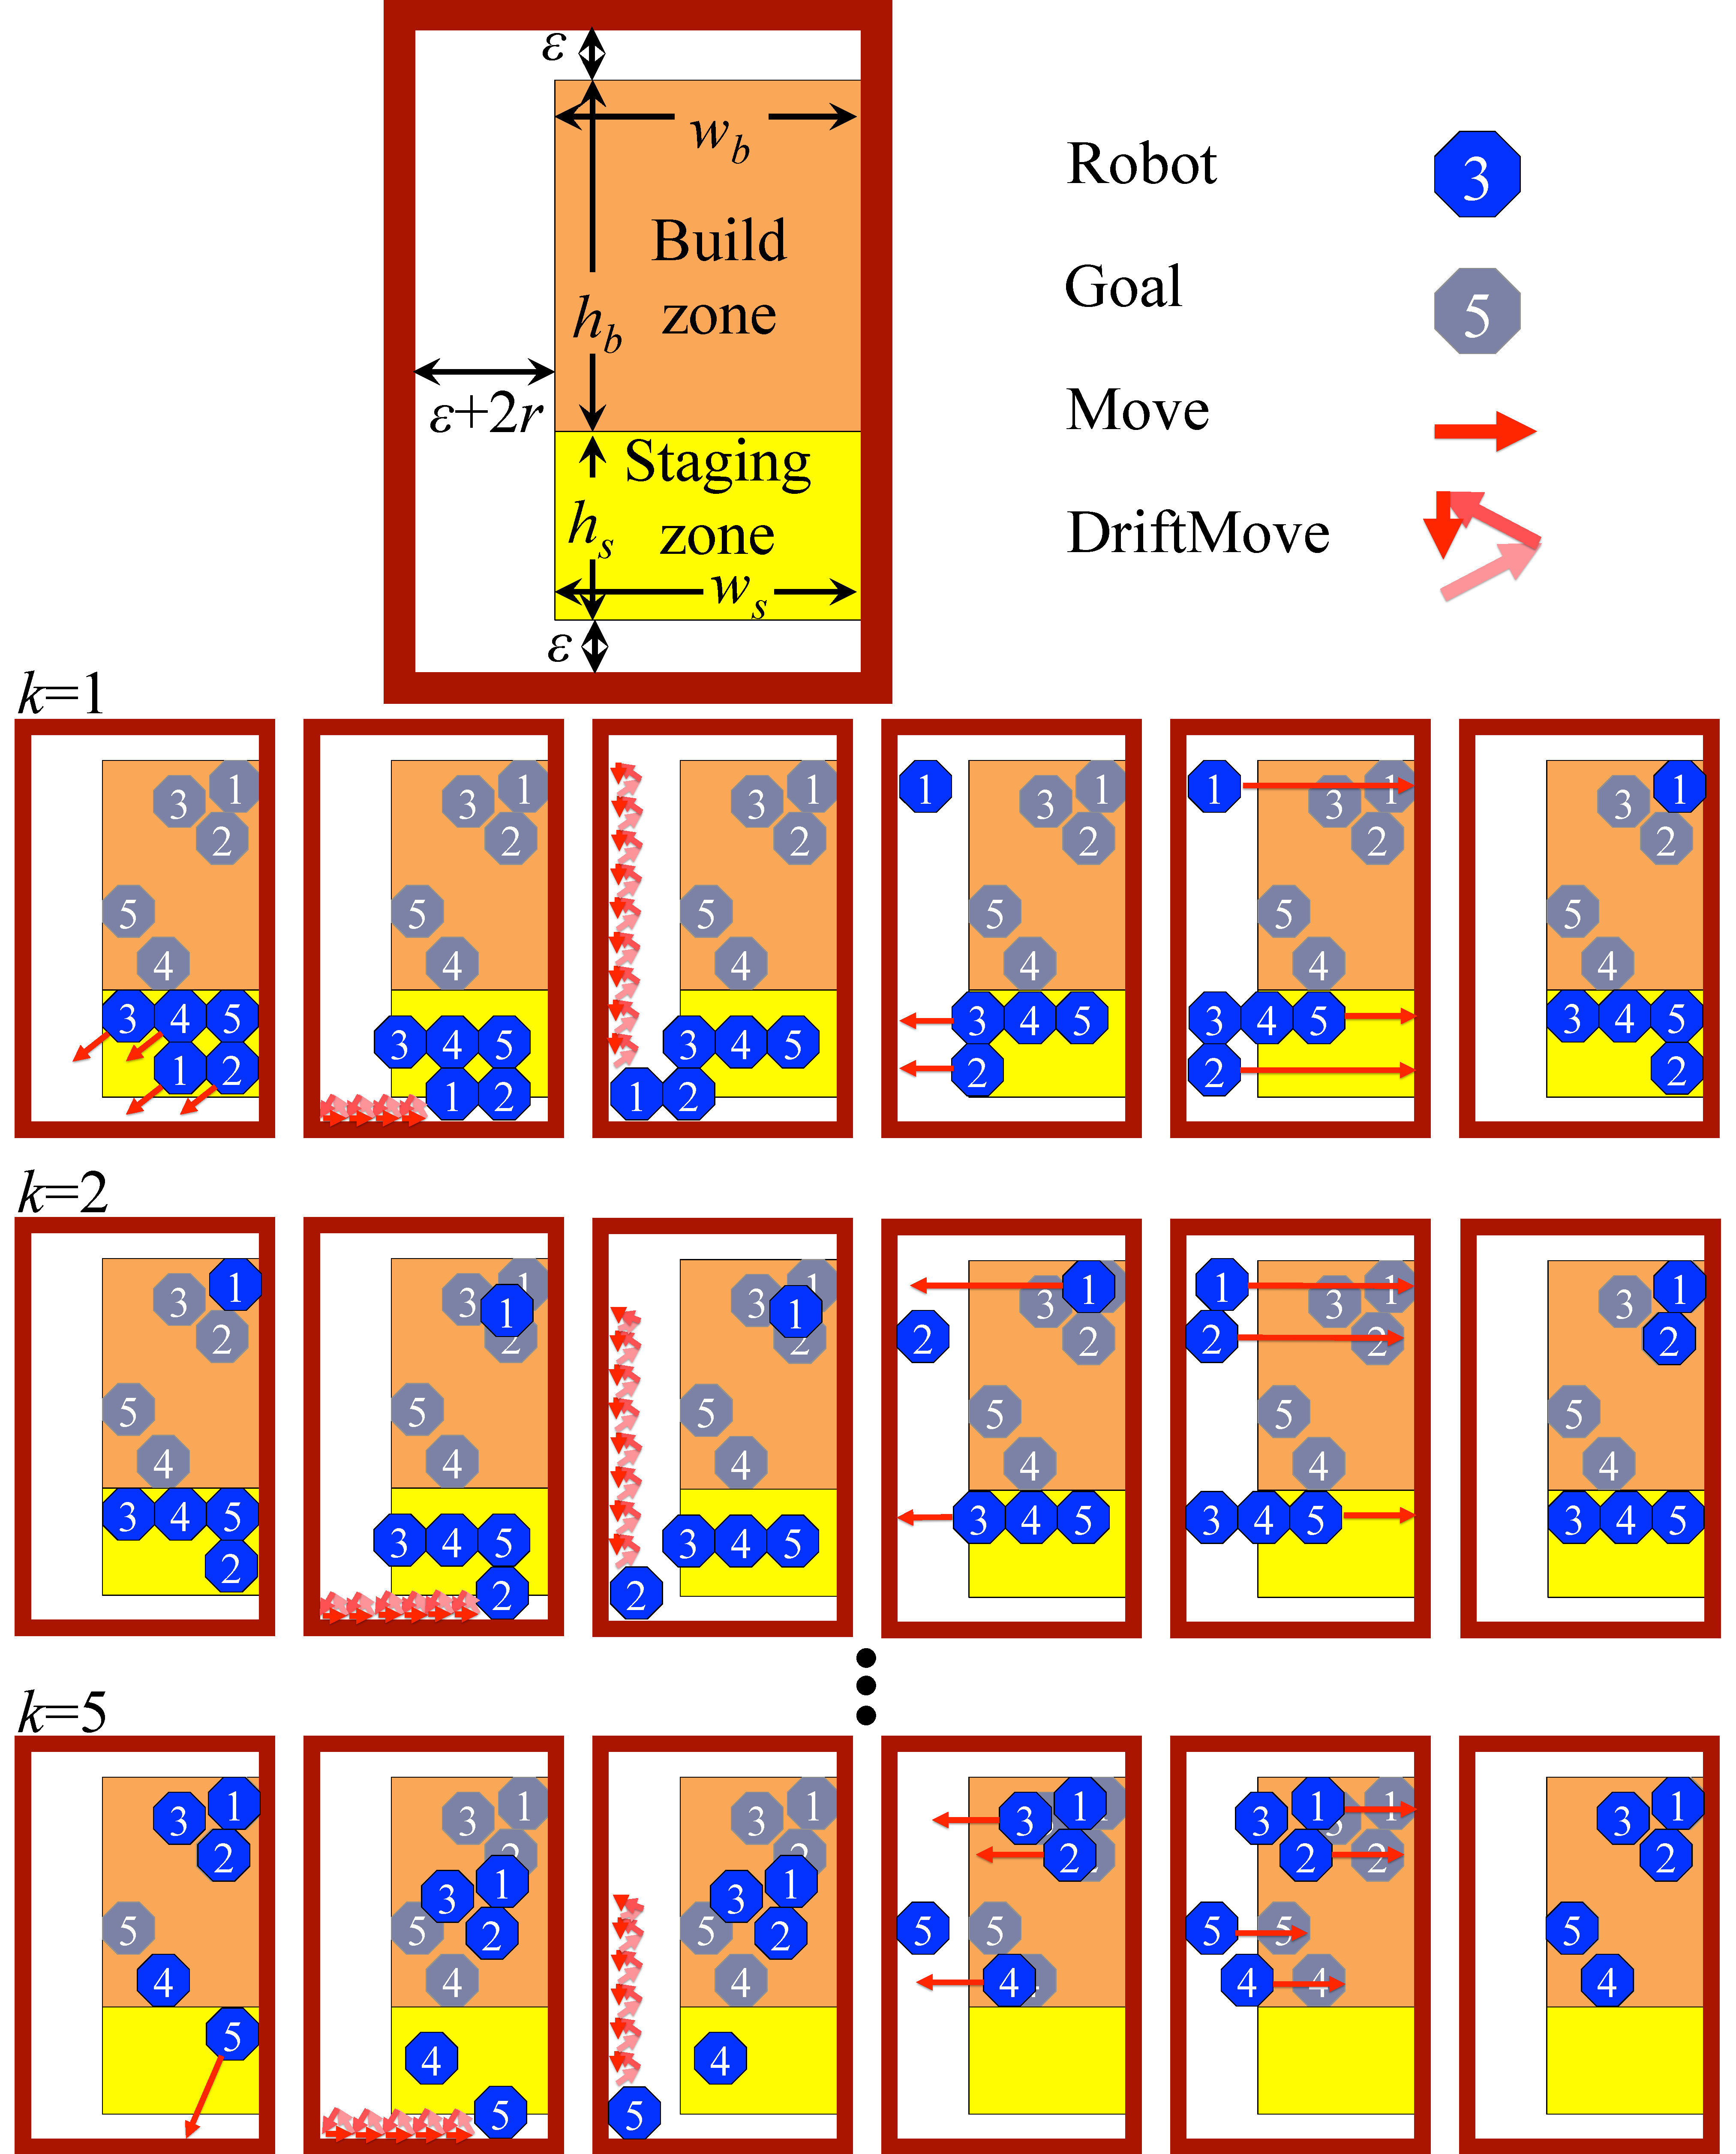
\includegraphics[width=1.0\columnwidth]{PositionNrobots.pdf}
\end{center}
\vspace{-1em}
\caption{\label{fig:simulationNrobot}
Illustration of Alg.\ \ref{alg:PosControlNRobots}, $n$ robot position control  using walls with non-slip contact.
}
\end{figure}

Assume an open workspace with four axis-aligned walls with non-slip contact.
The axis-aligned build zone of dimension $(w_b, h_b)$ containing the final configuration of $n$ robots must be disjoint from the axis-aligned staging zone of dimension $(w_s, h_s)$  containing the starting configuration of $n$ robots.
 Without loss of generality, assume the build zone  is above the staging zone.  Let $d$ be the diameter of the particles.
Furthermore, there must be at least $\epsilon$ space above the build zone, $\epsilon$ below the staging zone, and $\epsilon + d$ to the left of the build and staging zone.  The minimum workspace is then $(\epsilon + d + \max(w_b,w_s), 2\epsilon + h_s,h_b)$.

The $n$ robots position control algorithm relies on a $\text{\sc DriftMove}(\alpha, \beta, \epsilon,\theta)$ control input, described in Alg.~\ref{alg:DriftMove} and shown in Fig.\  \ref{fig:driftmove}.
For $\theta = 0^\circ$, a drift move consists of repeating a triangular movement sequence $\{ (\beta/2,-\epsilon),(\beta/2,\epsilon),(-\alpha,0)\}$. 
 Any particle touching a top wall moves right $\beta$ units, while every particle not touching the top moves right $\beta-\alpha$.

\begin{figure}
\begin{center}
%
\includegraphics[width=.47\columnwidth]{driftmove0.pdf}
%	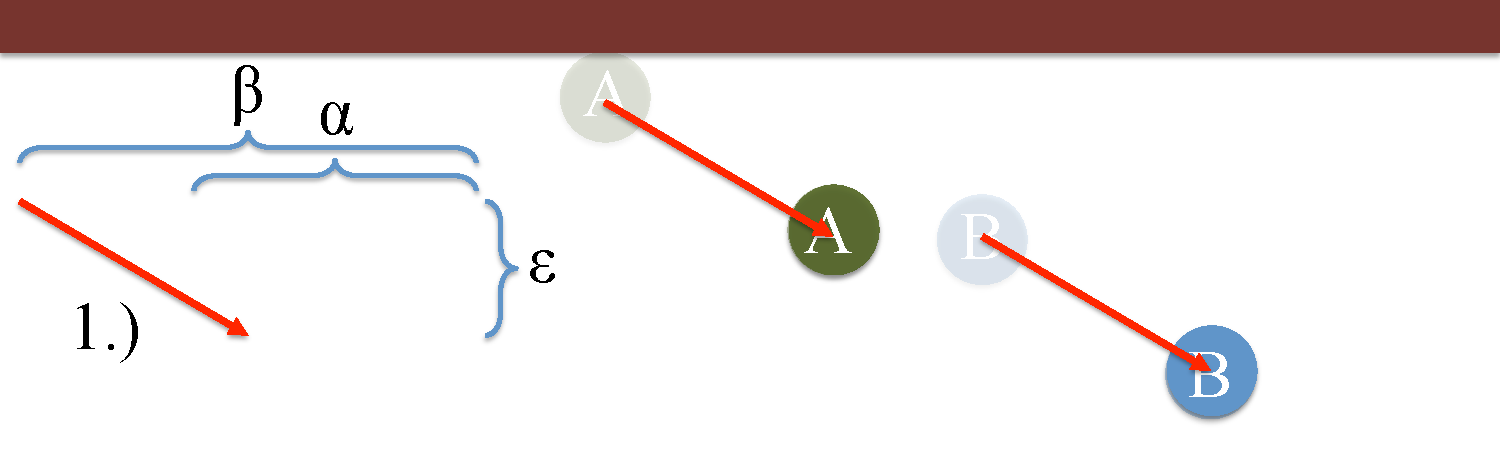
\includegraphics[width=.47\columnwidth]{driftmove1.pdf}
%	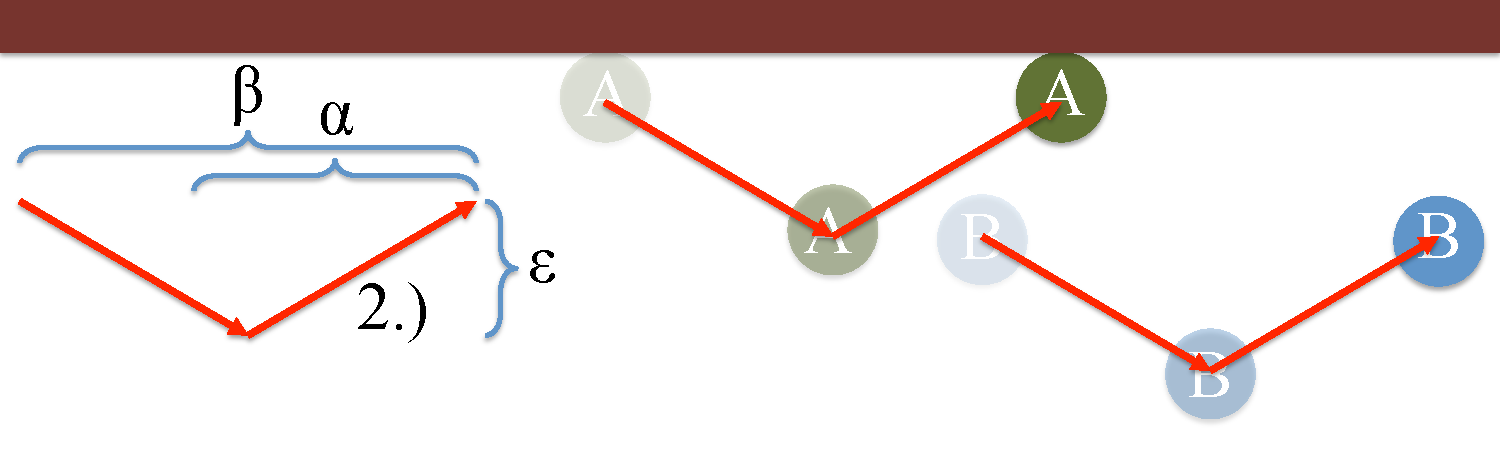
\includegraphics[width=.47\columnwidth]{driftmove2.pdf}
	\includegraphics[width=\columnwidth]{driftmovefullres.pdf}
\end{center}
\vspace{-1em}
\caption{\label{fig:driftmove}
A  $\text{\sc DriftMove}(\alpha, \beta, \epsilon,0^\circ)$ repeats a triangular movement sequence $\{ (\beta/2,-\epsilon)$, $(\beta/2,\epsilon)$, $(-\alpha,0)\}$. At the sequence end, robot $A$ has moved $\beta$ units right, and robot $B$ has moved $\beta-\alpha$ units right.}
\vspace{-1em}
\end{figure}

Let $(0,0)$ be the lower left corner of the workspace, $p_k$ the $x,y$ position of the $k^{\text{th}}$ robot, and $f_k$ the final $x,y$ position of the $k^{\text{th}}$ robot. Label the robots in the staging zone from left-to-right and bottom-to-top, and the $f_k$ configurations top-to-bottom and right-to-left as shown in Fig.~\ref{fig:construction2d}.

\begin{algorithm}
\caption{PositionControl$n$Robots($k$)}\label{alg:PosControlNRobots}
\begin{algorithmic}[1]
\State Move( $-\epsilon, d/2-p_{ky}$) % move  away from right wall and down till robot k touches bottom


\While{ $p_{kx} > d/2$} 
\State $\text{\sc DriftMove}(\epsilon, \min(p_{kx} - d/2,\epsilon), \epsilon,180^\circ)$    %drift move left until kth robot touches left wall
\EndWhile

\State $m \gets \operatorname{ceil}(\frac{f_{ky}-d/2}{\epsilon})$
\State $\beta \gets \frac{f_{ky}-d/2}{m}$
\State $\alpha \gets \beta - \frac{d/2 - p_{ky}-\epsilon}{m}$
\For{ $m$ iterations}
\State $\text{\sc DriftMove}(\alpha, \beta, \epsilon,90^\circ)$    %move kth robot to f_{ky} and leave the rest in position.
\EndFor

\State Move ($d/2+\epsilon-f_{kx}, 0$)  % move the group to the left until k is in the correct relative x position
\State Move ($f_{kx}-d/2, 0$)  

\end{algorithmic}
\end{algorithm}


\begin{algorithm}
\caption{ {\sc DriftMove}($\alpha,\beta,\epsilon,\theta$)
}\label{alg:DriftMove}
particles touching the wall move $\beta$ units, while particles not touching the wall move $\beta-\alpha$ units.
\begin{algorithmic}[1]
\State $R = \begin{bmatrix} \cos(\theta) & -\sin(\theta) \\
 \sin(\theta) & \cos(\theta)  \end{bmatrix}$
\State {\sc Move}$(R \cdot [\beta/2,-\epsilon]^\top)$ 
\State  {\sc Move}$(R \cdot [\beta/2,\epsilon]^\top)$ 
\State  {\sc Move}$(R \cdot [-\alpha,0]^\top)$ 
\end{algorithmic}
\end{algorithm}


Alg. \ref{alg:PosControlNRobots} proceeds as follows:  
First, the robots are moved left away from the right wall, and down so all robots in $k^{\text{th}}$ row touch the bottom wall.
Second, a set of $\operatorname{DriftMove}$s are executed that move all robots in $k^{\text{th}}$ row left until $k$ touches the left wall, with no net movement of the other robots.
Third, a set of $\operatorname{DriftMove}$s are executed that move only robot $k$ to its target height and return the other robots to their initial heights. 
Fourth, all robots except robot $k$ are pushed left until robot $k$ is in the correct relative $x$ position compared to robots 1 to $k-1$.
Finally, all robots are moved right until robot $k$ is in the desired target position. Running time is $O(n(w+h))$.



The hardware platform depicted in Fig.~\ref{fig:construction2d} is an assembled practical setup that assumes that $\epsilon= 1$ cm. 
The workspace is a $7\times 7$ cm grid space. 
All particles are 3D-printed plastic whose top is a 1cm diameter cylinder with a narrower base that encapsulates a steel bearing ball.
Non-slip wall contact is generated by a toothed wall design to keep particles from moving out of place while implementing the drift move. 
The workspace boundary is mounted on top of a white sheet of cardboard.
Underneath the cardboard, a grid of 3mm diameter magnets glued with 1 cm spacing to a thin board generates the uniform control input.
 A video attachment  shows the algorithm at work. 
This discretized setup requires several modifications to Alg.~\ref{alg:PosControlNRobots}.
 In this demonstration, all moves are 1 cm in length.
   All drift moves are a counterclockwise \emph{square} move  of size 1 cm$\times$1 cm. 
   Once the $k^{\text{th}}$ particle gets to its designated location in each loop, a correction step is implemented. 
   This correction step increases by two the total number of moves required per particle.
   Fig.~\ref{fig:simulationNrobot} shows there are only 6 stages per particle involved in Alg.~\ref{alg:PosControlNRobots}.
The fixed step algorithm requires 8 stages per particle as shown in Fig.~\ref{fig:construction2d}. 

A significant difference between Alg.~\ref{alg:PosControlNRobots} and the fixed move implementation of it is that Alg.~\ref{alg:PosControlNRobots}
enables placing particles at arbitrary, non-overlapping locations, while the fixed move implementation requires goal locations at the center of grid cells. 

\begin{figure}
\begin{center}
	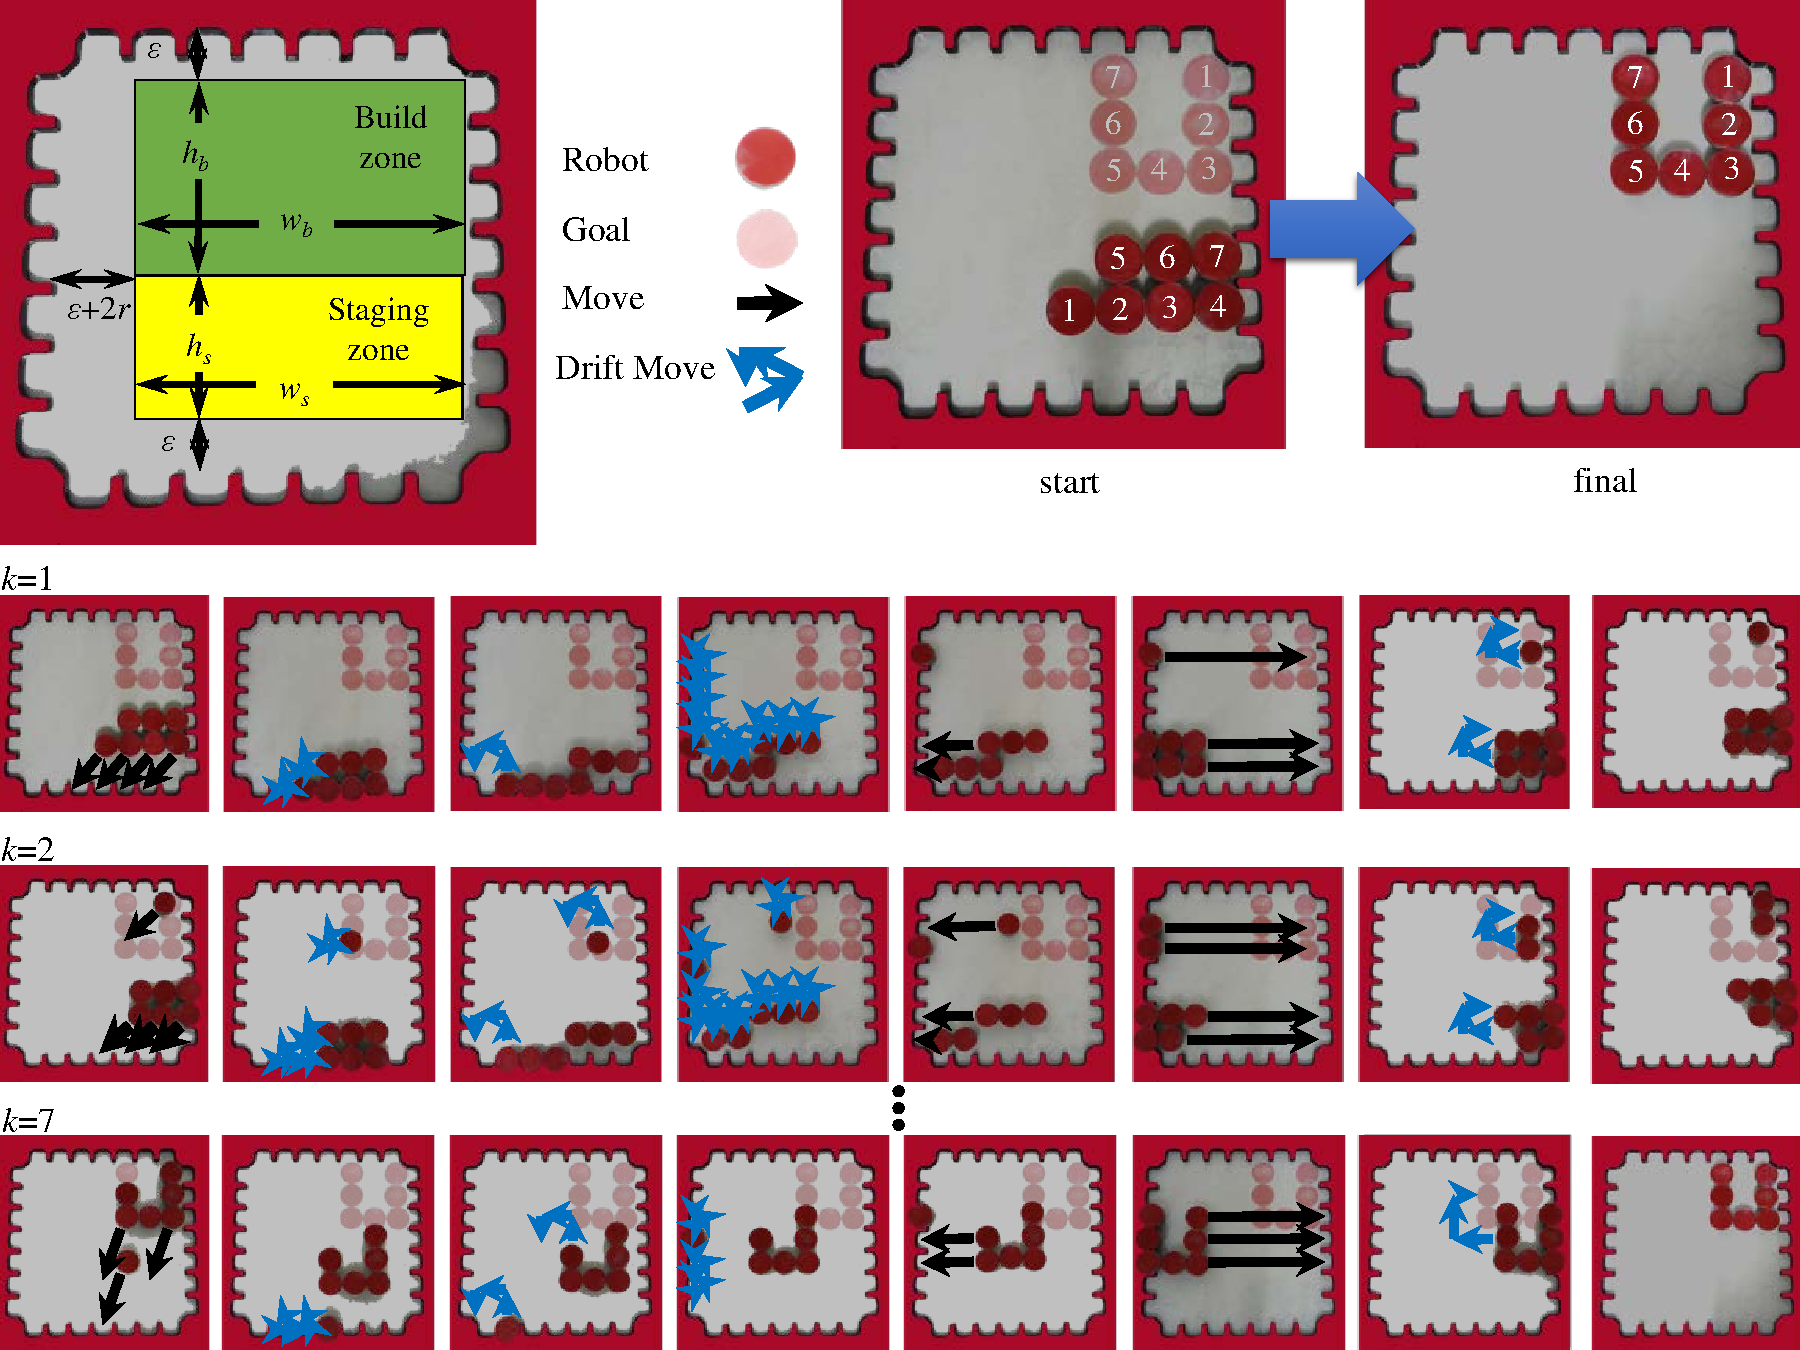
\includegraphics[width=1.0\columnwidth]{multirobotSliderHardware2.pdf}
\end{center}
\vspace{-1em}
\caption{\label{fig:construction2d}
Illustration of Alg.\ \ref{alg:PosControlNRobots}, discretized $n$ robot position control  using walls that enforce non-slip contact.
}
\end{figure}


%%%%%%%%%%%%%%%
%%%%%%%%%%%%%%%

\section{Simulation}\label{sec:simulation}


%Two simulations were implemented using non-slip contact walls for position control.  The first controls the position of two robots, the second controls the position of $n$ robots.  

%\subsection{Position Control of Two Robots}
\begin{figure}
\centering
\begin{overpic}[width=0.49\columnwidth]{worstnum.pdf}\put(0,75){a)}\end{overpic}
\begin{overpic}[width=0.49\columnwidth]{worstdist.pdf}\put(0,75){b)}\end{overpic}
\begin{overpic}[width=0.49\columnwidth]{middlegoalnum.pdf}\put(0,75){c)}\end{overpic}
\begin{overpic}[width=0.49\columnwidth]{middlegoaldist.pdf}\put(0,75){d)}\end{overpic}
\caption{\label{fig:contour}
Plots show performance with one goal on the boundary.
}
\end{figure}

\begin{figure}
\centering
%\begin{overpic}[width=\columnwidth]{deltanum.pdf}\end{overpic}\\
%\vspace{1em}
\begin{overpic}[width=\columnwidth]{deltadist.pdf}\end{overpic}
\vspace{-1em}
\caption{\label{fig:deltanumdist}
The worst case path length occurs when particles must swap antipodes. This can never be achieved but can be asymptotically approached. Plot shows decreasing error as the number of moves grows.
} 
\end{figure}


\begin{figure}
\centering
\renewcommand{\figwid}{1\columnwidth}
{
\begin{overpic}[width =\figwid]{contourDistnew.png}\put(-2,10){\begin{turn}{90} \tiny{unique particles}
\end{turn}}

\end{overpic}
\vspace{1em}
\begin{overpic}[width =\figwid]{JustSimulationV6.png}\put(-2,10){\begin{turn}{90} \tiny{unique particles}
\end{turn}}

\end{overpic}
\begin{overpic}[width =\figwid]{identical.png}\put(-2,6){\begin{turn}{90} \tiny{interchangeable particles}
\end{turn}}
\end{overpic}
}\caption{\label{fig:contourPlots}{Starting positions of particles $1$ and $2$ and goal position of particle $2$ are fixed, and $\epsilon=0.001$.
 The top row of contour plots show the distance if robot $1$'s goal position is varied in $x$ and $y$. The bottom row shows the number of moves required for the same configurations.}
\vspace{-1em}
}
\end{figure}
Algorithm \ref{alg:optimalAlg}  was implemented in Mathematica using particles with zero radius. 
%An online interactive demonstration and source code of the algorithm are available at \cite{Shahrokhi2015mathematicaParticle}.
%  Fig.~\ref{fig:shapeControlMathematica1}  shows  an implementation of this algorithm with robot initial positions represented by hollow squares and final positions by circles. 
 %Dashed lines show the shortest route if robots could be controlled independently, while solid lines show the optimal shortest  path using uniform inputs.
 
 The contour plots in Fig.~\ref{fig:contour} left show the length of the path for two different settings. Top row considers \{$s_1,s_2,g_1$\} = \{$(0.2,0.2),(-0.1,-0.1),(-0.2,0)$\} and bottom row considers  \{$s_1,s_2,g_1$\} = \{$(0.2,0.2),(-0.1,-0.1),(0,0)$\} in a workspace with $r= 0.5$, and $g_2$ ranging over all the workspace. Fig.~\ref{fig:contour} right shows the total distance of the path. This plot shows the nonlinear nature of the path planning. The path length grows when the goals have $\pi$ difference and are very close to the boundary. TODO:???? We need to discuss the new plots.
 The worst case occurs when the ending points are at antipodes along the boundary ($\pi$ angular distance). This can never be achieved but can be asymptotically approached as shown in Fig.~\ref{fig:deltanumdist}. 
 Fig.~\ref{fig:contourPlots} shows the same concepts in a square workspace. Fig.~\ref{fig:contourPlots} top and middle row considers the particles for three arbitrary starting and goal positions for the particles. All of the discussed plots have considered the particles to be unique. If particles are interchangeable and it does not matter to put the specific particle to its goal location, the path length will be significantly smaller. The bottom row of  Fig.~\ref{fig:contourPlots} considers interchangeable particles with the same configuration as the middle row with unique particles.
 
 %If the length of each side of the square workspace is $L$, the worst case path length is $(\sqrt{2}+2)L$.
 
% The plots in Fig.~\ref{fig:deltanumdist} show the exponentially increasing number of moves and distance when the accuracy of reaching to the goal ($\delta$) is getting to zero when the goal positions have $\pi$ difference with each on the boundaries.











%%%%%%%%%%%%%%%
%%%%%%%%%%%%%%%
%%%%%%%%%%%%%%%%%%%%%%%%%%%%%%%%%%%%%%%%%%%%%%%%%%%%%%%%%%%
\section{Experimental Results}\label{sec:expResults}
%%%%%%%%%%%%%%%%%%%%%%%%%%%%%%%%%%%%%%%%%%%%%%%%%%%%%%%%%%%
\begin{figure*}[htb!]\label{fig:3dPrinted}
\centering
\vspace{1.5em}
%\begin{overpic}[width=\columnwidth]{firstImage.jpg}\end{overpic}
\begin{overpic}[width=2\columnwidth]{3dexperiment.pdf}\end{overpic}
\\
\vspace{1em}
\begin{overpic}[width=2\columnwidth]{realTripe.pdf}\end{overpic}
\caption{\label{fig:story}
Frames showing particle positions before and after control inputs. Top row: small intestine phantom. Bottom row: cow stomach tissue.
} \vspace{-1em}
\end{figure*}

To demonstrate Alg.~\ref{alg:optimalAlg} experimentally, we performed several tests.
Each used the same magnetic setup shown in Fig.~\ref{fig:IntroPic}.
% The figure might need to be referenced 
 Two different intestine models were employed, the first a 3D-printed cross-section representation of a small intestine, and the second a cross-section of a bovine stomach.
 
 \subsection{Magnetic Manipulation Setup}
 
 The magnetic manipulation system has two pairs of electromagnetic coils, each with iron cores at their centers, and arranged orthogonal to each other. The iron core at the center of each coil concentrates the magnetic field towards the workspace. An Arduino and four SyRen regenerative motor drivers were used for control inputs to the coils. Finally, a FOculus F0134SB 659 x 494 pixel camera was attached to the top of the system, focusing on the workspace which was backlit by a $\SI{15}{\watt}$ LED light strip. 
 
To obtain experimental data, the test samples (the phantom intestine model and the bovine cross section) were placed in laser-cut acrylic discs and then immersed in corn syrup. Corn syrup was used to increase the viscosity to 12000 cP for the experiments. Spherical $\SI{1}{\milli\metre}$ magnets (supermagnetman \#SP0100-50) were used as our particles. Our experimental setup did not perfectly implement the system dynamics in \eqref{eq:swarmDynamicsAndFric}. In particular, the magnetic field in this setup is only approximately uniform. The magnetic force varies in both magnitude and orientation. As shown in the video attachment, this non-uniformity causes the particle closer to the coil to move faster than the other particle. This phenomenon makes it easier to increase particle separation than to decrease separation, but this can be compensated because boundary collisions easily decrease the separation. Also, magnetic forces are not exactly parallel, but point toward the center of the activated coil. Algorithm~\ref{alg:optimalAlg} still works despite these non-uniformities, but sometimes requires additional iterations.
 
%explain the magnetic field strength used, the camera system (briefly)
%explain the particles used

%explain the fluid used in the model.

\subsection{Intestine Phantom Model}

The intestine phantom model was used first and was made to mimic the geometry of an intestine and its villi. The model consists of a circular ring with an outer diameter of $\SI{50}{\milli\metre}$, an inner diameter of $\SI{46}{\milli\metre}$, and 60 $\SI{2}{\milli\metre}$ long protrusions on its inner surface cut out of $\SI{6}{\milli\metre}$ thick acrylic to model the geometry of intestinal villi. Figure \ref{fig:story} top row shows an experiment. Starting and ending positions were printed beneath the workspace on transparency film. Our algorithm successfully delivered the particles to goal positions in 10 out of 10 trials.

%methodology: we used xx material, built a model xx big


%todo: snapshots of the the beads in the model, moving toward goal.  We can add lots of annotations.  %Fake this series so we have an image for now.


\subsection{Bovine Stomach Cross-section}
%todo: procedure for fixating the Bovine tissue sample,
%discussion of the challenges 

Strips of cow stomach approximately $\SI{5}{\milli\metre}$ thick were cut and sewn to acrylic cylinder and then glued to an acrylic substrate using cyanoacrylate (superglue). This assembly was then filled with corn syrup. The experiment is shown in Fig.~\ref{fig:story} bottom row. Our algorithm successfully delivered the particles to goal positions in 5 out of 5 trials.
A video showing one trial of this experiment is available in the supplementary materials. 
%In using the small intestines, which were about 25mm in diameter, the resulting workspace was less than half of that of our simulated intestines. This meant more care had to be taken in navigating the magnets to their goal locations to avoid getting them too close to each other. 

%todo: snapshots of the the beads in the model, moving toward goal.  We can add lots of annotations.  Fake this series so we have an image for now.



%%%%%%%%%%%%%%%
%%%%%%%%%%%%%%%%%%%%%%%%%%%%%%%%%%%%%%%%%%%%%%%%%%%%%%%%%%%
\section{Conclusion and Future Work}\label{sec:conclusion}
%%%%%%%%%%%%%%%%%%%%%%%%%%%%%%%%%%%%%%%%%%%%%%%%%%%%%%%%%%%

This paper presented techniques for controlling the shape of a swarm of robots using uniform global inputs and interaction with boundary friction forces.  
The paper provided algorithms for precise position control, as well as robust and efficient covariance control. 
Extending algorithms \ref{alg:PosControl2Robots} and \ref{alg:PosControlNRobots}  to 3D is straightforward but increases the complexity.
Future efforts should be directed toward improving the technology and tailoring it to specific robot applications.

  With regard to technological advances, this includes designing controllers that efficiently regulate $\sigma_{xy}$, perhaps using Lyapunov-inspired controllers as in \citep{kim2015imparting}. 
 Additionally, this paper assumed nearly infinite wall friction.  The algorithms require retooling to handle small $\mu_f$ friction coefficients.  It may be possible to rank controllability as a function of friction.
%  In hardware, the wall friction can be varied by laser-cutting boundary walls with different of profiles. 
  
    

%TODO JOURNAL: design controllers that efficiently regulate $\sigma_{xy}$.
%TODO JOURNAL: We will design Lyapunov-inspired controllers for $\sigma_{xy}$ to prove controllability. 
%TODO JOURNAL:  and rank controllability as a function of friction.
% TODO: JOURNAL: and vary wall friction by laser-cutting boundary walls with a variety of profiles. 


%    Inspired by large-scale human experiments with swarms of robots under global control,  this paper investigated controllers that use only the mean and variance of a robot swarm. We proved that the mean position is controllable, and provided conditions under which variance is controllable.  We derived automatic controllers for each and a hysteresis-based switching control that controls the mean and variance of a robot swarm.  We employed these controllers as primitives for a block-pushing task. 
%    
%    Future work should implement these controllers on a robot swarm and decrease completion time by avoiding counter-productive contact with the block while the swarm is lowering its variance.  We have also assumed the swarm is unimodal and has a straight-line path to the moveable block. Relaxing these assumptions requires solving the \emph{gathering problem}.  The gathering problem for a swarm with uniform inputs is largely unexplored, and must be examined probabilistically for nontrivial environments.
%    
    % We should also control the covariance $\sigma_xy$ and higher moments of the distribution
    
    
    
%Sensing is expensive, especially on the nanoscale. To see nanocars~\citep{Chiang2011}, scientists fasten molecules that fluoresce light when activated by a strong light source. Unfortunately, multiple exposures can destroy these molecules, a process called \emph{photobleaching}. Photobleaching can be minimized by lowering the excitation light intensity, but this increases the probability of missed detections~\citep{Cazes2001}. A control methodology based on statistics of the robot swarm rather than the actual position of each robot, allows relaxing demands on imagine systems, controllers robust to tracking errors, and a simpler methodology.  In this work we...
%


% Additionally, as population characteristics, they are available even if only a percentage of the robots are detected each control cycle.
%Photobleaching: http://www.piercenet.com/browse.cfm?fldID=4DD9D52E-5056-8A76-4E6E-E217FAD0D86B
%
%Photobleaching is caused by the irreversible destruction of fluorophores due to either the prolonged exposure to the excitation source or exposure to high-intensity excitation light. Photobleaching can be minimized or avoided by exposing the fluor(s) to the lowest possible level of excitation light intensity for the shortest length of time that still yields the best signal detection; this requires optimization of the detection method using high sensitivity CCD cameras, high numerical aperture objective and/or the widest bandpass emission filter(s) available. Other approaches include using fluorophores that are more photostable than traditional fluorophores and/or using antifade reagents to protect the fluor(s) against photobleaching. Steps to avoid photobleaching are not feasible for all detection methods and should be optimized for each method used. For example, antifade reagents are toxic to live cells, and therefore they can only be used with fixed cells or tissue. Furthermore, some detection methods, such as flow cytometry, normally do not require steps to avoid photobleaching because of the extremely short exposure time of the fluorophore to the excitation source.
%%%%%%%%%%%%%%%
%\section*{Acknowledgments}
%%%%%%%%%%%%%%%
%% Use plainnat to work nicely with natbib. 
{%\footnotesize
%\bibliographystyle{plainnat}
%\bibliographystyle{SageH}
\bibliographystyle{IEEEtran}
\bibliography{IEEEabrv,SwarmShapeControl}
}

% Uncomment to add appendix:
%
\documentclass[conference]{IEEEtran}
\usepackage{times}

% numbers option provides compact numerical references in the text. 
\usepackage[numbers]{natbib}
\usepackage{multicol}
\usepackage[bookmarks=true]{hyperref}

\usepackage{bbm}
\usepackage{calc}
\usepackage{url}
\usepackage{hyperref}
\hypersetup{
  colorlinks =true,
  urlcolor = black,
  linkcolor = black
}
\usepackage{graphicx}
\usepackage[cmex10]{amsmath}
\usepackage{bm}
\usepackage{amssymb}
\usepackage{rotating}


%\usepackage{xfrac}
\usepackage{nicefrac}
\usepackage{cite}
\usepackage[caption=false,font=footnotesize]{subfig}
\usepackage[usenames, dvipsnames]{color}
\usepackage{colortbl}
%\usepackage{caption}

%\usepackage{wrapfig}
\usepackage{overpic}
%\usepackage{subfigure}
%\usepackage{textcomp}
\graphicspath{{./pictures/pdf/},{./pictures/ps/},{./pictures/png/},{./pictures/jpg/}}
\usepackage{breqn} %for breaking equations automatically
\usepackage[ruled]{algorithm}
\usepackage{algpseudocode}
%\usepackage{algorithmic}
\usepackage{multirow}
\usepackage{todonotes}

%\newcommand{\todo}[1]{\vspace{5 mm}\par \noindent \framebox{\begin{minipage}[c]{0.98 \columnwidth} \ttfamily\flushleft \textcolor{red}{#1}\end{minipage}}\vspace{5 mm}\par}
% uncomment this to hide all red todos
%\renewcommand{\todo}{}

%% ABBREVIATIONS
\newcommand{\qstart}{q_{\text{start}}}
\newcommand{\qgoal}{q_{\text{goal}}}
\newcommand{\pstart}{p_{\text{start}}}
\newcommand{\pgoal}{p_{\text{goal}}}
\newcommand{\xstart}{x_{\text{start}}}
\newcommand{\xgoal}{x_{\text{goal}}}
\newcommand{\ystart}{y_{\text{start}}}
\newcommand{\ygoal}{y_{\text{goal}}}
\newcommand{\gammastart}{\gamma_{\text{start}}}
\newcommand{\gammagoal}{\gamma_{\text{goal}}}
\providecommand{\proc}[1]{\textsc{#1}}


\newcommand{\ARLfull}{Aero\-space Ro\-bot\-ics La\-bora\-tory }
\newcommand{\ARL}{\textsc{arl}}
\newcommand{\JPL}{\textsc{jpl}}
\newcommand{\PRM}{\textsc{prm}}

\newcommand{\CM}{\textsc{cm}}
\newcommand{\SVM}{\textsc{svm}}
\newcommand{\NN}{\textsc{nn}}
\newcommand{\prm}{\textsc{prm}}
\newcommand{\lemur}{\textsc{lemur}}
\newcommand{\Lemur}{\textsc{Lemur}}
\newcommand{\LP}{\textsc{lp}} 
\newcommand{\SOCP}{\textsc{socp}}
\newcommand{\SDP}{\textsc{sdp}}
\newcommand{\NP}{\textsc{np}}
\newcommand{\SAT}{\textsc{sat}}
\newcommand{\LMI}{\textsc{lmi}}
\newcommand{\hrp}{\textsc{hrp\nobreakdash-2}}
\newcommand{\DOF}{\textsc{dof}}
\newcommand{\UIUC}{\textsc{uiuc}}
%% MACROS


\providecommand{\abs}[1]{\left\lvert#1\right\rvert}
\providecommand{\norm}[1]{\left\lVert#1\right\rVert}
\providecommand{\normn}[2]{\left\lVert#1\right\rVert_#2}
\providecommand{\dualnorm}[1]{\norm{#1}_\ast}
\providecommand{\dualnormn}[2]{\norm{#1}_{#2\ast}}
\providecommand{\set}[1]{\lbrace\,#1\,\rbrace}
\providecommand{\cset}[2]{\lbrace\,{#1}\nobreak\mid\nobreak{#2}\,\rbrace}
\providecommand{\lscal}{<}
\providecommand{\gscal}{>}
\providecommand{\lvect}{\prec}
\providecommand{\gvect}{\succ}
\providecommand{\leqscal}{\leq}
\providecommand{\geqscal}{\geq}
\providecommand{\leqvect}{\preceq}
\providecommand{\geqvect}{\succeq}
\providecommand{\onevect}{\mathbf{1}}
\providecommand{\zerovect}{\mathbf{0}}
\providecommand{\field}[1]{\mathbb{#1}}
\providecommand{\C}{\field{C}}
\providecommand{\R}{\field{R}}
\newcommand{\Cspace}{\mathcal{Q}}
\newcommand{\Uspace}{\mathcal{U}}
\providecommand{\Fspace}{\Cspace_\text{free}}
\providecommand{\Hcal}{$\mathcal{H}$}
\providecommand{\Vcal}{$\mathcal{V}$}
\DeclareMathOperator{\conv}{conv}
\DeclareMathOperator{\cone}{cone}
\DeclareMathOperator{\homog}{homog}
\DeclareMathOperator{\domain}{dom}
\DeclareMathOperator{\range}{range}
\DeclareMathOperator{\sign}{sgn}
\providecommand{\polar}{\triangle}
\providecommand{\ainner}{\underline{a}}
\providecommand{\aouter}{\overline{a}}
\providecommand{\binner}{\underline{b}}
\providecommand{\bouter}{\overline{b}}
\newcommand{\D}{\nobreakdash-\textsc{d}}
%\newcommand{\Fspace}{\mathcal{F}}
\providecommand{\Fspace}{\Cspace_\text{free}}
\providecommand{\free}{\text{\{}\mathsf{free}\text{\}}}
\providecommand{\iff}{\Leftrightarrow}
\providecommand{\subinner}[1]{#1_{\text{inner}}}
\providecommand{\subouter}[1]{#1_{\text{outer}}}
\providecommand{\Ppoly}{\mathcal{X}}
\providecommand{\Pproj}{\mathcal{Y}}
\providecommand{\Pinner}{\subinner{\Pproj}}
\providecommand{\Pouter}{\subouter{\Pproj}}
\DeclareMathOperator{\argmax}{arg\,max}
\providecommand{\Aineq}{B}
\providecommand{\Aeq}{A}
\providecommand{\bineq}{u}
\providecommand{\beq}{t}
\DeclareMathOperator{\area}{area}
\newcommand{\contact}[1]{\Cspace_{#1}}
\newcommand{\feasible}[1]{\Fspace_{#1}}
\newcommand{\dd}{\; \mathrm{d}}
\newcommand{\figwid}{0.22\columnwidth}
\newcommand{\TRUE}{\textbf{true}}
\newcommand{\FALSE}{\textbf{false}}
\DeclareMathOperator{\atan2}{atan2}


\newtheorem{theorem}{Theorem}
\newtheorem{definition}[theorem]{Definition}
\newtheorem{lemma}[theorem]{Lemma}


\pdfinfo{
   /Author (Shiva Shahrokhi, Arun Mahadev, and Aaron T. Becker)
   /Title  (Supplement toAlgorithms For Shaping a Particle Swarm With a Shared Control Input Using Boundary Interaction)
   /CreationDate (D:20160129120000)
   /Subject (Simple Robots)
   /Keywords (Robots;Uniform Control Inputs)
}

\begin{document}

% paper title
\title{\huge{ \emph{Supplement to} 
Algorithms For Shaping a Particle Swarm\\ With a Shared Control Input Using Boundary Interaction}}

\author{Shiva Shahrokhi, Arun Mahadev, and Aaron T. Becker}


\maketitle

\begin{abstract}
%Also 
Includes algorithms and equations too lengthy for main paper, but potentially useful for the community.
Also links to videos and demonstration code for the algorithms.

Consider a swarm of agents that are controlled by the same global inputs and have no autonomy. This paper presents algorithms for shaping such swarms in 2D.

This model is common for current micro- and nano-robots, whose small size makes it difficult to perform onboard computation or contain a power and propulsion source. For this reason these robots are usually powered and controlled by global inputs, such as a uniform external electric or magnetic field, and every robot receives exactly the same control inputs.
Due to their small size, large numbers of micro-robots are required to deliver sufficient payloads.
 Nevertheless, these applications require precision control of the shape and position of the robot swarm. Precision control requires breaking the symmetry caused by the global input.  

A promising technique uses collisions with boundary walls to shape the swarm, however, the range of configurations created by conforming a swarm to a boundary wall is limited. This paper describes the set of stable configurations of a swarm in two canonical workspaces, a circle and a square. 

To increase the diversity of configurations, we add boundary interaction to our model.  We provide algorithms using friction with walls to place two robots at arbitrary locations in a rectangular workspace.
Next, we extend this algorithm to place $n$ robots at desired locations. We conclude with efficient techniques to control the covariance of a swarm not possible without wall-friction. Simulations and hardware implementations with 100 robots validate these results.

\end{abstract}

\IEEEpeerreviewmaketitle

\section{Introduction}
This supplement gives overviews of the videos and code in 
\S \ref{sec:Videos}, 
provides the algorithm for $y$ position control of two robots in
\S \ref{sec:2robotWallFriction},
and gives gull analytical models for fluid settling in square-shaped tanks in
\S \ref{sec:fluidInPlanarRegion}.


\section{Supplementary Videos}\label{sec:Videos}
Five videos animate the key algorithms in this paper.

\subsection{Robot Swarm in a Circle under Gravity}
The video \emph{Robot Swarm in a Circle under Gravity} shows the stable configuration of a swarm under a constant global input.  Animated plots show mean, variance, covariance, and correlation for a swarm in a circular workspace.
Full resolution video: \url{https://youtu.be/nPFAjVIOxYc}.
An online demonstration and source code of the algorithm are at \citet{Zhao2016mathematicaSquare}.

\subsection{Distribution of Robot Swarm in Square under Gravity }
The video \emph{Distribution of Robot Swarm in Square under Gravity } shows the stable configuration of a swarm under a constant global input.  Animated plots show mean, variance, covariance, and correlation for a swarm in a square workspace.
Full resolution video: \url{https://youtu.be/ZEksDxLpAzg}.
An online demonstration and source code of the algorithm are at \citet{Zhao2016mathematica}.


\subsection{Steering 2 Particles with Shared Controls Using Wall Friction}
Animates Algs. 1, 2, 3 in Mathematica to show how two robots can be arbitrarily positioned in a square workspace. In this video the desired initial and ending positions of the two robots are manipulated, and the path that the robots should follow is drawn. The video ends with an extreme case where the robots must exchange positions. 
Full resolution video: \url{https://youtu.be/5TWlw7vThsM}.
An online demonstration and source code of the algorithm are at \citet{Shahrokhi2015mathematicaParticle}.

\subsection{Arranging a robot swarm with global inputs and wall friction [discrete] }
An implementation of Alg. 4  in {\sc Matlab} that illustrates how the two robots positioning algorithm is extendable to $n$ robots. In this video all  robots gets the same input, but by exploiting wall friction each robot reaches its goal, the formation "UH".
Full resolution video: \url{https://youtu.be/uhpsAyPwKeI}.
Full code is available at \citet{Arun2015}.
Note that this code uses discretized version of Algorithm 3.  The continuous-movement version is illustrated in Fig.\ref{PositionNrobots.pdf}.
\begin{figure}
\begin{center}
	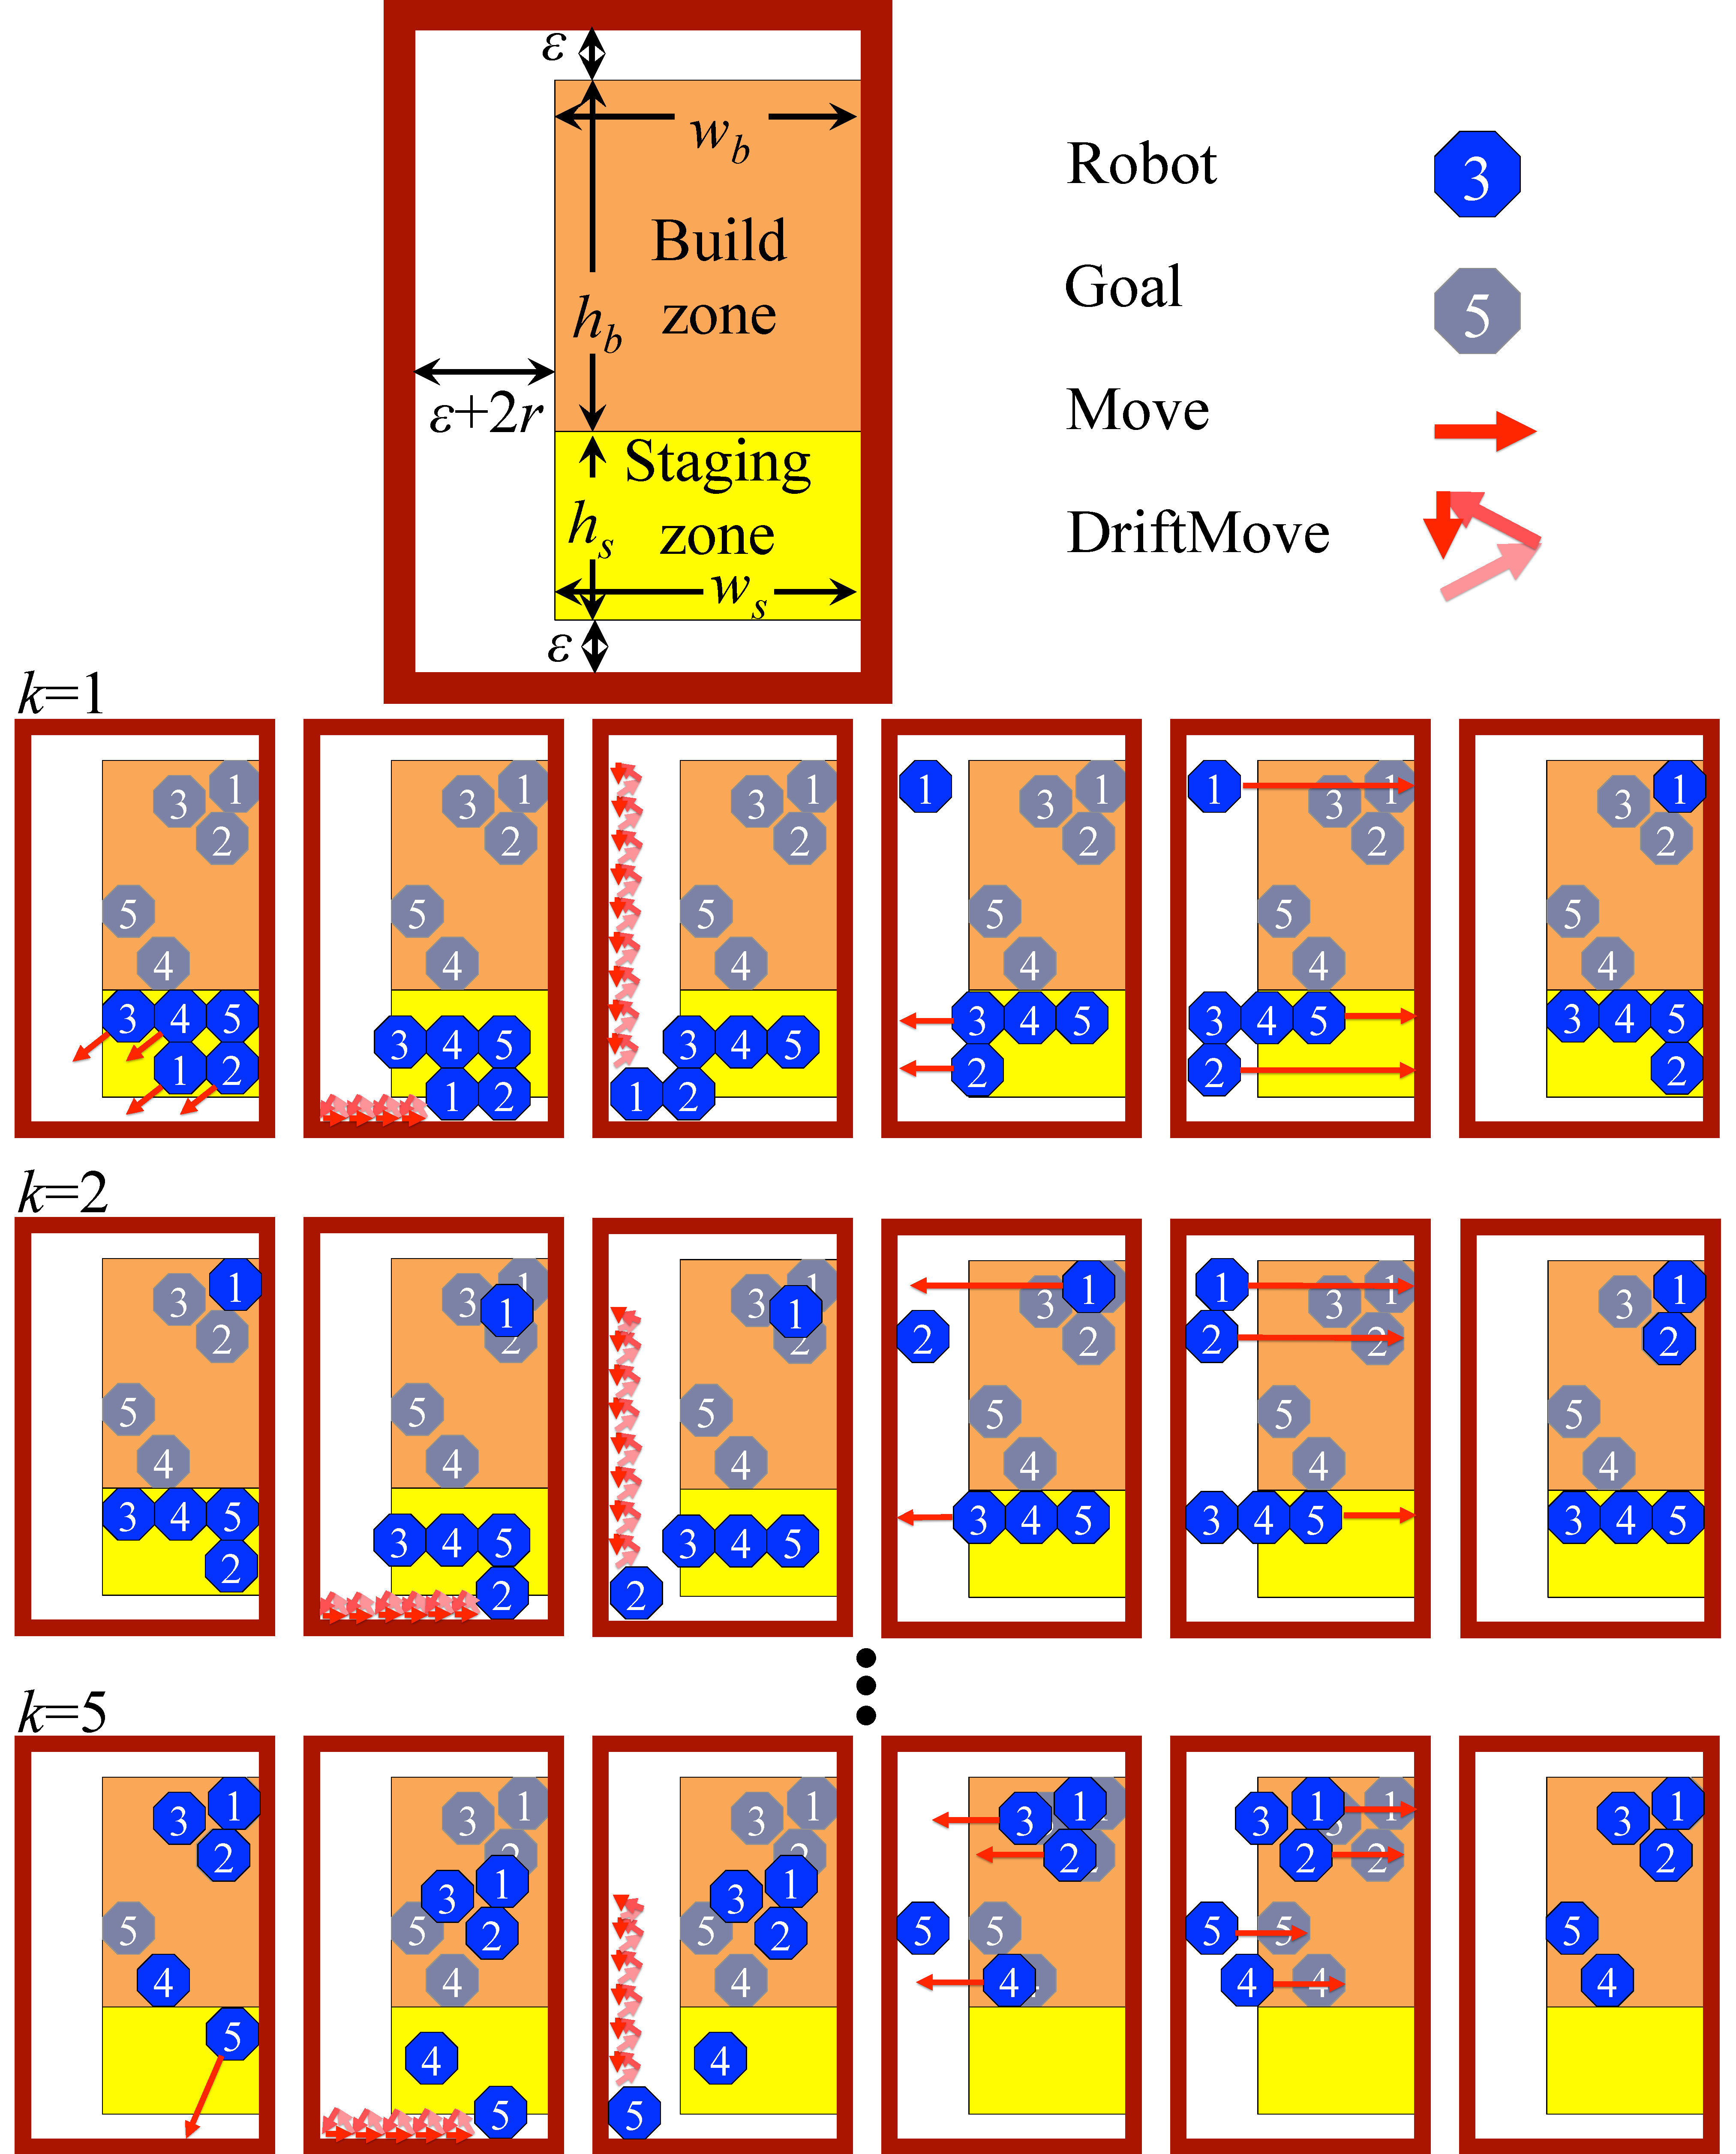
\includegraphics[width=1.0\columnwidth]{PositionNrobots.pdf}
\end{center}
\vspace{-1em}
\caption{\label{fig:construction2d}
Illustration of Alg.\ \ref{alg:PosControlNRobots}, $n$ robot position control  using wall friction.
}
\end{figure}




\subsection{AutomaticCovControl.mp4}
A closed-loop controller that steers a swarm of particles to a desired covariance,  implemented with a box2D simulator. In this video the green ellipse is the desired covariance ellipse, the red ellipse is the current covariance ellipse of the swarm and the red dot is the mean position of the robots. Robots follow the algorithm to achieve the desired values for $\sigma_{goalxy}$, $\sigma_x^2$ and $\sigma_y^2$.

%%%%%%%%%%%%%%%%%%%%%%%%%%%%%
\section{ Algorithm for generating desired $y$ spacing between two robots using wall friction}\label{sec:2robotWallFriction}
\begin{algorithm}
\caption{GenerateDesired$y$-spacing($s_1,s_2,e_1,e_2,L$)}\label{alg:YControl}
\begin{algorithmic}[1]
\Require Knowledge of starting $(s_1,s_2)$ and ending $(e_1,e_2)$ positions of  two robots. 
$(0,0)$ is bottom corner, $s_1$ is rightmost robot, 
 $L$ is length of the walls. Current position of the robots are $(r_1,r_2)$.
\Ensure   $ r_{1x} - r_{2x}  \equiv s_{1x} - s_{2x} $   %$\Delta y(t) \equiv \Delta y(0)$ 
\State $ \Delta s_y  \gets s_{1y} - s_{2y} $
\State $ \Delta e_y \gets e_{1y} - e_{2y} $
\State $ r_1 \gets s_1$, $ r_2 \gets s_2$
\If {$\Delta e_y < 0 $ }
\State $ m \gets ( L-\max( r_{1y},r_{2y}) ,0)   $ \Comment{Move to top wall}
\Else 
\State  $ m \gets ( -\min( r_{1y},r_{2y}),0 )    $ \Comment{Move to bottom wall}
\EndIf
\State $m  \gets  m + (0, -\min( r_{1x},r_{2x} ))$ \Comment{Move to left}
\State $ r_1 \gets r_1+m$, $ r_2 \gets r_2+m$ \Comment{Apply move}
\If {$\Delta e_y - (r_{1y} - r_{2y} ) > 0 $}
\State $ m \gets (\min(|\Delta e_y - \Delta s_y |, L- r_{1y}), 0)$  \Comment{Move top}
\Else
\State $ m \gets (-\min(|\Delta e_y - \Delta s_y |, r_{1y}), 0)$\Comment{Move bottom}
\EndIf 
\State $m  \gets  m + (0, \epsilon)$ \Comment{Move right}
\State $ r_1 \gets r_1+m$, $ r_2 \gets r_2+m$ \Comment{Apply move}
\State $\Delta r_y = r_{1y} - r_{2y}$
\If {$\Delta r_y \equiv \Delta e_y$} 
\State   $ m \gets (e_{1x}-r_{1x}, e_{1y}-r_{1y})$
\State $ r_1 \gets r_1+m$, $ r_2 \gets r_2+m$ \Comment{Apply move}
\State  \Return $(r_1,r_2)$
\Else   
\State \Return GenerateDesired$y$-spacing($r_1,r_2,e_1,e_2,L$)
\EndIf
\end{algorithmic}
\end{algorithm}



%%%%%%%%%%%%%%%%%%%%%%%%%%%
\section{Calculations for modeling swarm as fluid in a simple planar workspace}\label{sec:fluidInPlanarRegion}
Two workspaces are used, a square and a circular workspace.

\subsection{Square Workspace}
This section provides formulas for the mean, variance,  covariance and correlation of a very large swarm of robots as they move inside a square workplace under the influence of gravity pointing in the direction $\beta$. The swarm is large, but the robots are small in comparison, and together cover an area of constant volume $A$. Under a global input such as gravity, they flow like water, moving to a side of the workplace and forming a polygonal shape. The workspace is 

The range of possible angles for the global input angle $\beta $ is [0,2$\pi $). In this range of angles, the swarm assumes eight different polygonal shapes. The shapes alternate between triangles and trapezoids when the area $A$$<$1/2, and alternate between squares with one corner removed and trapezoids when $A$$>$1/2.

Two representative formulas are attached, the outline of the swarm shapes in \eqref{tab:SquareRobotRegions} and $\bar{x}(\beta,A)$ in \eqref{tab:SquareXMean}.




\begin{figure}[h]
\begin{center}
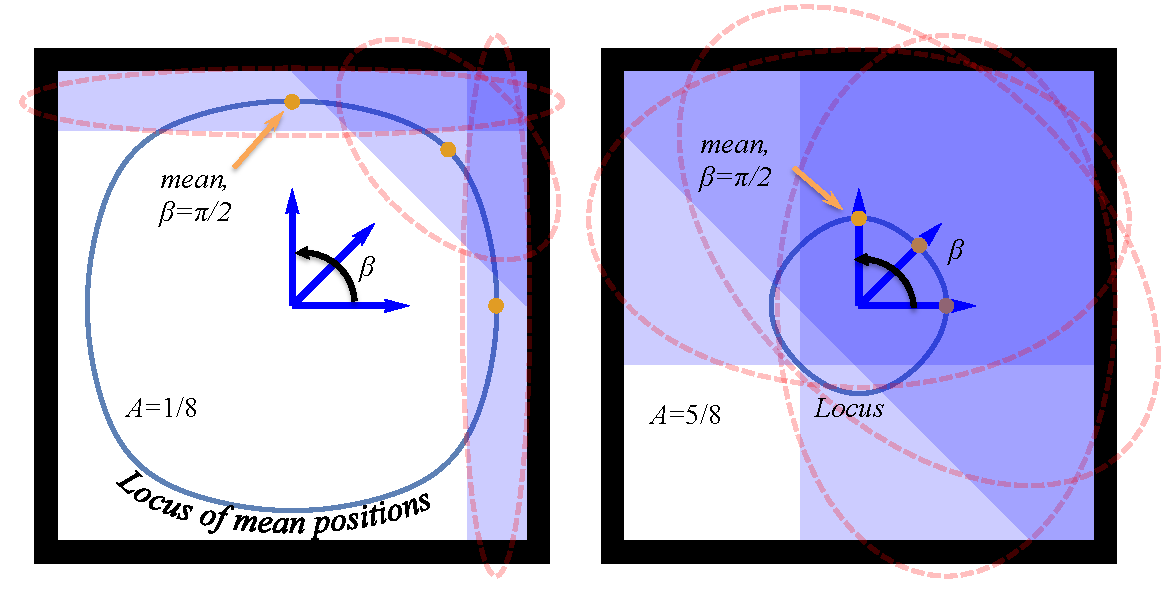
\includegraphics[width=\columnwidth]{SquarePlotPositions.pdf} 
\caption{A swarm in a square workspace under a constant global input assumes either a triangular or a trapezoidal shape if $A<1/2$.  If $A>1/2$ the swarm is either a squares with one corner removed or a trapezoidal  shape.}
\label{fig:friction}
\end{center}
\end{figure} 

\begin{table*}
\begin{align}
\bar{x}(\beta,A) = A\leq \frac{1}{2}: &\begin{cases}
 -\frac{\tan ^2(\beta )}{24 A}-\frac{A}{2}+1 & 0\leq \beta \leq \tan ^{-1}(2 A)\lor 2 \pi -\tan ^{-1}(2 A)<\beta \leq 2 \pi  \\
 1-\frac{1}{3} \sqrt{2} \sqrt{A \tan (\beta )} & \tan ^{-1}(2 A)<\beta \leq \frac{\pi }{2}-\tan ^{-1}(2 A) \\
 \frac{\cot (\beta )}{12 A}+\frac{1}{2} & \frac{\pi }{2}-\tan ^{-1}(2 A)<\beta \leq \tan ^{-1}(2 A)+\frac{\pi }{2} \\
 \frac{1}{3} \sqrt{2} \sqrt{-A \tan (\beta )} & \tan ^{-1}(2 A)+\frac{\pi }{2}<\beta \leq \pi -\tan ^{-1}(2 A) \\
 \frac{\tan ^2(\beta )}{24 A}+\frac{A}{2} & \pi -\tan ^{-1}(2 A)<\beta \leq \tan ^{-1}(2 A)+\pi  \\
 \frac{1}{3} \sqrt{2} \sqrt{A \tan (\beta )} & \tan ^{-1}(2 A)+\pi <\beta \leq \frac{3 \pi }{2}-\tan ^{-1}(2 A) \\
 \frac{1}{2}-\frac{\cot (\beta )}{12 A} & \frac{3 \pi }{2}-\tan ^{-1}(2 A)<\beta \leq \tan ^{-1}(2 A)+\frac{3 \pi }{2} \\
 1-\frac{1}{3} \sqrt{2} \sqrt{-A \tan (\beta )} & \tan ^{-1}(2 A)+\frac{3 \pi }{2}<\beta \leq 2 \pi -\tan ^{-1}(2 A) \\
\end{cases} \nonumber\\
\frac{1}{2}<A<1:&\begin{cases}
 -\frac{\tan ^2(\beta )}{24 A}-\frac{A}{2}+1 & 0\leq \beta \leq \tan ^{-1}\left(\frac{1}{2},1-A\right)\lor 2 \pi -\tan ^{-1}\left(\frac{1}{2},1-A\right)<\beta \leq 2 \pi  \\
 \frac{2 \sqrt{2} \sqrt{(1-A) \tan (\beta )} (A-1)+3}{6 A} & \tan ^{-1}\left(\frac{1}{2},1-A\right)<\beta \leq \frac{\pi }{2}-\tan ^{-1}\left(\frac{1}{2},1-A\right) \\
 \frac{6 A+\cot (\beta )}{12 A} & \frac{\pi }{2}-\tan ^{-1}\left(\frac{1}{2},1-A\right)<\beta \leq \tan ^{-1}\left(\frac{1}{2},1-A\right)+\frac{\pi }{2} \\
 \frac{-2 \sqrt{2} \sqrt{(A-1) \tan (\beta )} (A-1)+6 A-3}{6 A} & \tan ^{-1}\left(\frac{1}{2},1-A\right)+\frac{\pi }{2}<\beta \leq \pi -\tan ^{-1}\left(\frac{1}{2},1-A\right) \\
 \frac{\tan ^2(\beta )}{24 A}+\frac{A}{2} & \pi -\tan ^{-1}\left(\frac{1}{2},1-A\right)<\beta \leq \tan ^{-1}\left(\frac{1}{2},1-A\right)+\pi  \\
 \frac{2 \sqrt{2} \sqrt{(1-A) \tan (\beta )} (1-A)+6 A-3}{6 A} & \tan ^{-1}\left(\frac{1}{2},1-A\right)+\pi <\beta \leq \frac{3 \pi }{2}-\tan ^{-1}\left(\frac{1}{2},1-A\right) \\
 \frac{1}{2}-\frac{\cot (\beta )}{12 A} & \frac{3 \pi }{2}-\tan ^{-1}\left(\frac{1}{2},1-A\right)<\beta \leq \tan ^{-1}\left(\frac{1}{2},1-A\right)+\frac{3 \pi }{2} \\
 \frac{2 \sqrt{2} \sqrt{(A-1) \tan (\beta )} (A-1)+3}{6 A} & \tan ^{-1}\left(\frac{1}{2},1-A\right)+\frac{3 \pi }{2}<\beta \leq 2 \pi -\tan ^{-1}\left(\frac{1}{2},1-A\right) \\
\end{cases}
 \nonumber \\
A=1: &\frac{1}{2}
\end{align}
\protect\caption{$\bar{x}$ in a unit-square workspace}
\label{tab:SquareXMean}
\end{table*}



\begin{table*}
\tiny
\begin{align}
\text{RobotRegion}(\beta,A)= \nonumber 
A\leq \frac{1}{2}:&
\begin{cases}
 \left(
\begin{array}{cc}
 1 & 0 \\
 1 & 1 \\
 -A-\frac{\tan (\beta )}{2}+1 & 1 \\
 -A+\frac{\tan (\beta )}{2}+1 & 0 \\
\end{array}
\right) & 0\leq \beta \leq \tan ^{-1}(2 A)\lor 2 \pi -\tan ^{-1}(2 A)<\beta \leq 2 \pi  \\
 \left(
\begin{array}{cc}
 1 & 1 \\
 1-\sqrt{2} \sqrt{A \tan (\beta )} & 1 \\
 1 & 1-\sqrt{2} \sqrt{A \cot (\beta )} \\
\end{array}
\right) & \tan ^{-1}(2 A)<\beta \leq \frac{\pi }{2}-\tan ^{-1}(2 A) \\
 \left(
\begin{array}{cc}
 1 & 1 \\
 0 & 1 \\
 0 & -A+\frac{\cot (\beta )}{2}+1 \\
 1 & -A-\frac{\cot (\beta )}{2}+1 \\
\end{array}
\right) & \frac{\pi }{2}-\tan ^{-1}(2 A)<\beta \leq \tan ^{-1}(2 A)+\frac{\pi }{2} \\
 \left(
\begin{array}{cc}
 0 & 1 \\
 \sqrt{2} \sqrt{-A \tan (\beta )} & 1 \\
 0 & 1-\sqrt{2} \sqrt{-A \cot (\beta )} \\
\end{array}
\right) & \tan ^{-1}(2 A)+\frac{\pi }{2}<\beta \leq \pi -\tan ^{-1}(2 A) \\
 \left(
\begin{array}{cc}
 0 & 0 \\
 0 & 1 \\
 A-\frac{\tan (\beta )}{2} & 1 \\
 A+\frac{\tan (\beta )}{2} & 0 \\
\end{array}
\right) & \pi -\tan ^{-1}(2 A)<\beta \leq \tan ^{-1}(2 A)+\pi  \\
 \left(
\begin{array}{cc}
 0 & 0 \\
 0 & \sqrt{2} \sqrt{A \cot (\beta )} \\
 \sqrt{2} \sqrt{A \tan (\beta )} & 0 \\
\end{array}
\right) & \tan ^{-1}(2 A)+\pi <\beta \leq \frac{3 \pi }{2}-\tan ^{-1}(2 A) \\
 \left(
\begin{array}{cc}
 0 & 0 \\
 1 & 0 \\
 1 & A-\frac{\cot (\beta )}{2} \\
 0 & A+\frac{\cot (\beta )}{2} \\
\end{array}
\right) & \frac{3 \pi }{2}-\tan ^{-1}(2 A)<\beta \leq \tan ^{-1}(2 A)+\frac{3 \pi }{2} \\
 \left(
\begin{array}{cc}
 1 & 0 \\
 1-\sqrt{2} \sqrt{-A \tan (\beta )} & 0 \\
 1 & \sqrt{2} \sqrt{-A \cot (\beta )} \\
\end{array}
\right) & \tan ^{-1}(2 A)+\frac{3 \pi }{2}<\beta \leq 2 \pi -\tan ^{-1}(2 A) \\
\end{cases}
 %%%%%%%%%%%%%%%%%%%%%%%%%%%%%%%%%%
\nonumber \\
\frac{1}{2}<A<1:&
\begin{cases}
 \left(
\begin{array}{cc}
 1 & 0 \\
 1 & 1 \\
 (1-A)-\frac{\tan (\beta )}{2} & 1 \\
 (1-A)+\frac{\tan (\beta )}{2} & 0 \\
\end{array}
\right) & 0\leq \beta \leq \tan ^{-1}\left(\frac{1}{2},1-A\right)\lor 2 \pi -\tan ^{-1}\left(\frac{1}{2},1-A\right)<\beta \leq 2 \pi  \\
 \left(
\begin{array}{cc}
 1 & 0 \\
 1 & 1 \\
 0 & 1 \\
 0 & \sqrt{2} \sqrt{(1-A) \cot (\beta )} \\
 \sqrt{2} \sqrt{(1-A) \tan (\beta )} & 0 \\
\end{array}
\right) & \tan ^{-1}\left(\frac{1}{2},1-A\right)<\beta \leq \frac{\pi }{2}-\tan ^{-1}\left(\frac{1}{2},1-A\right) \\
 \left(
\begin{array}{cc}
 0 & 1 \\
 1 & 1 \\
 1 & (1-A)-\frac{\cot (\beta )}{2} \\
 0 & (1-A)+\frac{\cot (\beta )}{2} \\
\end{array}
\right) & \frac{\pi }{2}-\tan ^{-1}\left(\frac{1}{2},1-A\right)<\beta \leq \tan ^{-1}\left(\frac{1}{2},1-A\right)+\frac{\pi }{2} \\
 \left(
\begin{array}{cc}
 1 & 1 \\
 0 & 1 \\
 0 & 0 \\
 1-\sqrt{2} \sqrt{-(1-A) \tan (\beta )} & 0 \\
 1 & \sqrt{2} \sqrt{-(1-A) \cot (\beta )} \\
\end{array}
\right) & \tan ^{-1}\left(\frac{1}{2},1-A\right)+\frac{\pi }{2}<\beta \leq \pi -\tan ^{-1}\left(\frac{1}{2},1-A\right) \\
 \left(
\begin{array}{cc}
 0 & 0 \\
 0 & 1 \\
 -(1-A)-\frac{\tan (\beta )}{2}+1 & 1 \\
 -(1-A)+\frac{\tan (\beta )}{2}+1 & 0 \\
\end{array}
\right) & \pi -\tan ^{-1}\left(\frac{1}{2},1-A\right)<\beta \leq \tan ^{-1}\left(\frac{1}{2},1-A\right)+\pi  \\
 \left(
\begin{array}{cc}
 1 & 0 \\
 0 & 0 \\
 0 & 1 \\
 1-\sqrt{2} \sqrt{(1-A) \tan (\beta )} & 1 \\
 1 & 1-\sqrt{2} \sqrt{(1-A) \cot (\beta )} \\
\end{array}
\right) & \tan ^{-1}\left(\frac{1}{2},1-A\right)+\pi <\beta \leq \frac{3 \pi }{2}-\tan ^{-1}\left(\frac{1}{2},1-A\right) \\
 \left(
\begin{array}{cc}
 1 & 0 \\
 0 & 0 \\
 0 & -(1-A)+\frac{\cot (\beta )}{2}+1 \\
 1 & -(1-A)-\frac{\cot (\beta )}{2}+1 \\
\end{array}
\right) & \frac{3 \pi }{2}-\tan ^{-1}\left(\frac{1}{2},1-A\right)<\beta \leq \tan ^{-1}\left(\frac{1}{2},1-A\right)+\frac{3 \pi }{2} \\
 \left(
\begin{array}{cc}
 0 & 0 \\
 1 & 0 \\
 1 & 1 \\
 \sqrt{2} \sqrt{-(1-A) \tan (\beta )} & 1 \\
 0 & 1-\sqrt{2} \sqrt{-(1-A) \cot (\beta )} \\
\end{array}
\right) & \tan ^{-1}\left(\frac{1}{2},1-A\right)+\frac{3 \pi }{2}<\beta \leq 2 \pi -\tan ^{-1}\left(\frac{1}{2},1-A\right) \\
\end{cases},\nonumber\\
%%%%%%%%%%%%%%%%%%%%%%%%%%%%%%%
A=1:&\left(
\begin{array}{cc}
 1 & 0 \\
 0 & 0 \\
 0 & 1 \\
 1 & 1 \\
\end{array}
\right)
\end{align}
\protect\caption{RobotRegions in a unit-square workspace}
\label{tab:SquareRobotRegions}
\end{table*}


\subsection{Circle Workspace}
The area under a chord of a circle is the area of a sector less the area of the triangle originating at the circle center: 
$A=S(sector)-S(triangle)=1/2 LR-1/2 C(1-h)$, thus
\begin{align}
A=(1/2)\left[LR-c(R-h)\right]
\end{align}
where $L$ is arc length, $c$ is chord length, $R$ is radius and $h$ is height. Solving for $L$ and $C$ gives
\begin{align}
L&=2 \cos ^{-1}(1-h)\\
C&=2\sqrt{h(2-h)}
\end{align}
Therefore the area under a chord is
\begin{align}
\cos ^{-1}(1-h)-(1-h) \sqrt{(2-h) h}
\end{align}

For a circular workspace, with $\beta = 0$, the variance of $x$ and $y$ are:
{\tiny
\begin{align}
&\sigma_x^2(h)=\frac{64 (h-2)^3 h^3}{144 \left(\sqrt{-(h-2) h} (h-1)+\arccos(1-h)\right)^2} +\nonumber\\
&\frac{9 \left(\sqrt{-(h-2) h} (h-1)+\arccos(1-h)\right) \left(\sin \left(4 \arcsin(1-h)\right)+4 \arccos(1-h)\right)}{144 \left(\sqrt{-(h-2) h} (h-1)+\arccos(1-h)\right)^2}
\end{align}}

{\tiny
\begin{align}
\sigma_y^2(h)=
\frac{12 \arccos(1-h)-8 \sin \left(2 \arccos(1-h)\right)+\sin \left(4 \arccos(1-h)\right)}{48 \left(\sqrt{-(h-2) h} (h-1)+\arccos(1-h)\right)}
\end{align}}

For $\beta = 0$, $\sigma_{xy}=0$. These values can be rotated to calculate $\sigma_x^2(\beta,h),\sigma_y^2(\beta,h),$ and $\sigma_{xy}(\beta,h)$.

%%%%%%%%%%%%%%%%%%%%%%%%%%%%%%
\section*{Acknowledgments}
This work was supported by the National Science Foundation under Grant No.\ \href{http://nsf.gov/awardsearch/showAward?AWD_ID=1553063}{ [IIS-1553063]}.

%%%%%%%%%%%%%%%
%% Use plainnat to work nicely with natbib. 
\bibliographystyle{plainnat}
\footnotesize
\bibliography{IEEEabrv,ShapingSwarmFrictionSharedInput}
\end{document}





\end{document}